\RequirePackage[l2tabu,orthodox]{nag}

% TODO: decide if one-sided/two-sided
%\documentclass[headsepline,footsepline,footinclude=false,fontsize=11pt,paper=a4,listof=totoc,bibliography=totoc,BCOR=12mm,DIV=12]{scrbook} % two-sided % original source stated: BCOR=12mm,DIV=12
\documentclass[headsepline,footsepline,footinclude=false,oneside,fontsize=11pt,paper=a4,listof=totoc,bibliography=totoc,DIV=12]{scrbook} % one-sided
\usepackage{wrapfig}
\usepackage{graphicx}
\usepackage{listings}
\usepackage{xcolor}
\usepackage{acronym}

\lstset{
    language=C++,                          
    basicstyle=\ttfamily\small,            
    %backgroundcolor=\color{lightgray},
    commentstyle=\color{gray},            
    keywordstyle=\color{blue}\bfseries,    % Style for keywords
    stringstyle=\color{orange},               % Style for strings
    numbers=left,                          % Line numbers on the left
    numberstyle=\tiny\color{gray},         % Style for line numbers
    stepnumber=1,                          % Number every line
    breaklines=true,                       % Break long lines
    frame=single,                          % Add a frame around the code
    breakatwhitespace=false,
    showspaces=false,
    rulecolor=\color{black},               % Color of the frame
    showstringspaces=false,                % Do not show spaces in strings
    showtabs=false,
    tabsize=2,                             % Tab size
    captionpos=b                           % Caption position: bottom
}

% TODO: change citation style in settings
\PassOptionsToPackage{table,svgnames,dvipsnames}{xcolor}

\usepackage[utf8]{inputenc}
\usepackage[T1]{fontenc}
\usepackage[sc]{mathpazo}
\usepackage[ngerman,english]{babel} % english is the same as american or USenglish
\usepackage[autostyle]{csquotes}
\usepackage[%
  backend=biber,
  url=true,
  style=numeric, % alphabetic, numeric
  sorting=none, % default == nty, https://tex.stackexchange.com/questions/51434/biblatex-citation-order
  maxnames=4,
  minnames=3,
  maxbibnames=99,
  giveninits,
  uniquename=init]{biblatex} % TODO: adapt citation style
\usepackage{graphicx}
\usepackage{scrhack} % necessary for listings package
\usepackage{listings}
\usepackage{lstautogobble}
\usepackage{tikz}
\usepackage{pgfplots}
\usepackage{pgfplotstable}
\usepackage{booktabs} % for better looking table creations, but bad with vertical lines by design (package creator despises vertical lines)
\usepackage[final]{microtype}
\usepackage{caption}
\usepackage[hidelinks]{hyperref} % hidelinks removes colored boxes around references and links
\usepackage{ifthen} % for comparison of the current language and changing of the thesis layout
\usepackage{pdftexcmds} % string compare to work with all engines
\usepackage{paralist} % for condensed enumerations or lists
\usepackage{subfig} % for having figures side by side
\usepackage{siunitx} % for physical accurate units and other numerical presentations
\usepackage{multirow} % makes it possible to have bigger cells over multiple rows in a table
\usepackage{array} % different options for table cell orientation
\usepackage{makecell} % allows nice manual configuration of cells with linebreaks in \thead and \makecell with alignments
\usepackage{pdfpages} % for including multiple pages of pdfs
\usepackage{adjustbox} % can center content wider than the \textwidth
\usepackage{tablefootnote} % for footnotes in tables as \tablefootnote
\usepackage{threeparttable} % another way to add footnotes as \tablenotes with \item [x] <your footnote> after setting \tnote{x} 


% https://tex.stackexchange.com/questions/42619/x-mark-to-match-checkmark
\usepackage{amssymb}% http://ctan.org/pkg/amssymb
\usepackage{pifont}% http://ctan.org/pkg/pifont
\newcommand{\cmark}{\ding{51}}%
\newcommand{\xmark}{\ding{55}}%


\usepackage[acronym,xindy,toc]{glossaries} % TODO: include "acronym" if glossary and acronym should be separated
\makeglossaries
\loadglsentries{pages/glossary.tex} % important update for glossaries, before document


\bibliography{bibliography}

\setkomafont{disposition}{\normalfont\bfseries} % use serif font for headings
\linespread{1.05} % adjust line spread for mathpazo font

% Add table of contents to PDF bookmarks
\BeforeTOCHead[toc]{{\cleardoublepage\pdfbookmark[0]{\contentsname}{toc}}}

% Define TUM corporate design colors
% Taken from http://portal.mytum.de/corporatedesign/index_print/vorlagen/index_farben
\definecolor{TUMBlue}{HTML}{0065BD}
\definecolor{TUMSecondaryBlue}{HTML}{005293}
\definecolor{TUMSecondaryBlue2}{HTML}{003359}
\definecolor{TUMBlack}{HTML}{000000}
\definecolor{TUMWhite}{HTML}{FFFFFF}
\definecolor{TUMDarkGray}{HTML}{333333}
\definecolor{TUMGray}{HTML}{808080}
\definecolor{TUMLightGray}{HTML}{CCCCC6}
\definecolor{TUMAccentGray}{HTML}{DAD7CB}
\definecolor{TUMAccentOrange}{HTML}{E37222}
\definecolor{TUMAccentGreen}{HTML}{A2AD00}
\definecolor{TUMAccentLightBlue}{HTML}{98C6EA}
\definecolor{TUMAccentBlue}{HTML}{64A0C8}

% Settings for pgfplots
\pgfplotsset{compat=newest}
\pgfplotsset{
  % For available color names, see http://www.latextemplates.com/svgnames-colors
  cycle list={TUMBlue\\TUMAccentOrange\\TUMAccentGreen\\TUMSecondaryBlue2\\TUMDarkGray\\},
}

% Settings for lstlistings

% Use this for basic highlighting
\lstset{%
  basicstyle=\ttfamily,
  columns=fullflexible,
  autogobble,
  keywordstyle=\bfseries\color{TUMBlue},
  stringstyle=\color{TUMAccentGreen}
}

% use this for C# highlighting
% %\setmonofont{Consolas} %to be used with XeLaTeX or LuaLaTeX
% \definecolor{bluekeywords}{rgb}{0,0,1}
% \definecolor{greencomments}{rgb}{0,0.5,0}
% \definecolor{redstrings}{rgb}{0.64,0.08,0.08}
% \definecolor{xmlcomments}{rgb}{0.5,0.5,0.5}
% \definecolor{types}{rgb}{0.17,0.57,0.68}

% \lstset{language=[Sharp]C,
% captionpos=b,
% %numbers=left, % numbering
% %numberstyle=\tiny, % small row numbers
% frame=lines, % above and underneath of listings is a line
% showspaces=false,
% showtabs=false,
% breaklines=true,
% showstringspaces=false,
% breakatwhitespace=true,
% escapeinside={(*@}{@*)},
% commentstyle=\color{greencomments},
% morekeywords={partial, var, value, get, set},
% keywordstyle=\color{bluekeywords},
% stringstyle=\color{redstrings},
% basicstyle=\ttfamily\small,
% }

% Settings for search order of pictures
\graphicspath{
    {logos/}
    {figures/}
}

% Set up hyphenation rules for the language package when mistakes happen
\babelhyphenation[english]{
an-oth-er
ex-am-ple
}

% Decide between
%\newcommand{\todo}[1]{\textbf{\textsc{\textcolor{TUMAccentOrange}{(TODO: #1)}}}} % for one paragraph, otherwise error!
%\newcommand{\done}[1]{\textit{\textsc{\textcolor{TUMAccentBlue}{(Done: #1)}}}} % for one paragraph, otherwise error!
% and
\newcommand{\todo}[1]{{\bfseries{\scshape{\color{TUMAccentOrange}[(TODO: #1)]}}}} % for multiple paragraphs
\newcommand{\done}[1]{{\itshape{\scshape{\color{TUMAccentBlue}[(Done: #1)]}}}} % for multiple paragraphs
% for error handling of intended behavior in your latex documents.

\newcommand{\tabitem}{~~\llap{\textbullet}~~}

\newcolumntype{P}[1]{>{\centering\arraybackslash}p{#1}} % for horizontal alignment with limited column width
\newcolumntype{M}[1]{>{\centering\arraybackslash}m{#1}} % for horizontal and vertical alignment with limited column width
\newcolumntype{L}[1]{>{\raggedright\arraybackslash}m{#1}} % for vertical alignment left with limited column width
\newcolumntype{R}[1]{>{\raggedleft\arraybackslash}m{#1}} % for vertical alignment right with limited column width

% TODO: change thesis information
\newcommand*{\getUniversity}{Technical University of Munich}
\newcommand*{\getFaculty}{School of Computation, Information and Technology - Informatics}
\newcommand*{\getTitle}{Hardware Abstraction of an ECU}
\newcommand*{\getTitleGer}{Hardware-Abstraktion einer ECU}
\newcommand*{\getAuthor}{Eslam Nasrallah}
\newcommand*{\getDoctype}{Bachelor's Thesis in Informatics}
\newcommand*{\getSupervisor}{Prof. Dr. Michael Gerndt}
\newcommand*{\getAdvisor}{M.Sc. Jianfeng Gu, Johannes Urlhardt}
\newcommand*{\getSubmissionDate}{30-09-2024}
\newcommand*{\getSubmissionLocation}{Munich}

\begin{document}

% TODO: decide on used language
%\selectlanguage{ngerman}
\selectlanguage{english}

% Set page numbering to avoid "destination with the same identifier has been already used" warning for cover page.
% (see https://en.wikibooks.org/wiki/LaTeX/Hyperlinks#Problems_with_Links_and_Pages).
\pagenumbering{alph}
\begin{titlepage}
  % HACK for two-sided documents: ignore binding correction for cover page.
  % Adapted from Markus Kohm's KOMA-Script titlepage=firstiscover handling.
  % See http://mirrors.ctan.org/macros/latex/contrib/koma-script/scrkernel-title.dtx,
  % \maketitle macro.
  \oddsidemargin=\evensidemargin\relax
  \textwidth=\dimexpr\paperwidth-2\evensidemargin-2in\relax
  \hsize=\textwidth\relax

  \centering

  \IfFileExists{logos/tum.pdf}{%
    
\includegraphics[height=20mm]{logos/tum.pdf}
  }{%
    \vspace*{20mm}
  }

  \vspace{5mm}
  {\huge\MakeUppercase{\getFaculty{}}}\\

  \vspace{5mm}
  {\large\MakeUppercase{\getUniversity{}}}\\

  \vspace{20mm}
  {\Large \getDoctype{}}

  \vspace{15mm}
  \makeatletter
  \ifthenelse{\pdf@strcmp{\languagename}{english}=0}
  {\huge\bfseries \getTitle{}}
  {\huge\bfseries \getTitleGer{}}
  \makeatother

  \vspace{15mm}
  {\LARGE \getAuthor{}}

  \IfFileExists{logos/faculty.png}{%
    \vfill{}
    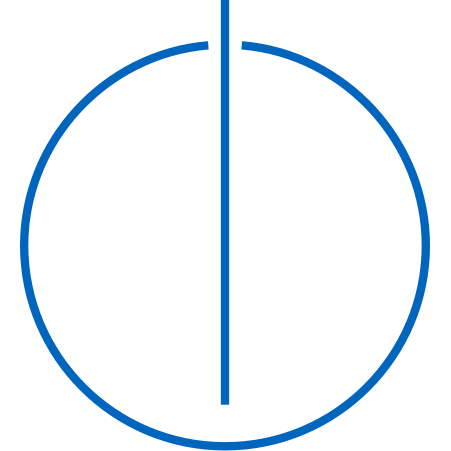
\includegraphics[height=20mm]{logos/faculty.png}
  }{}
\end{titlepage}


\frontmatter{}

\begin{titlepage}
  \centering

  \IfFileExists{logos/tum.pdf}{%
    
\includegraphics[height=20mm]{logos/tum.pdf}
  }{%
    \vspace*{20mm}
  }

  \vspace{5mm}
  {\huge\MakeUppercase{\getFaculty{}}}\\

  \vspace{5mm}
  {\large\MakeUppercase{\getUniversity{}}}\\

  \vspace{20mm}
  {\Large \getDoctype{}}

  \makeatletter
  \vspace{15mm}
  \ifthenelse{\pdf@strcmp{\languagename}{english}=0}
  {
  {\huge\bfseries \getTitle{}}

  \vspace{10mm}
  {\huge\bfseries \foreignlanguage{ngerman}{\getTitleGer{}}}
  }
  {
  {\huge\bfseries \getTitleGer{}}

  \vspace{10mm}
  {\huge\bfseries \foreignlanguage{english}{\getTitle{}}}
  }
  \makeatother

  \vspace{15mm}
  \begin{tabular}{l l}
    Author:          & \getAuthor{} \\
    Supervisor:      & \getSupervisor{} \\
    Advisor:         & \getAdvisor{} \\
    Submission Date: & \getSubmissionDate{} \\
  \end{tabular}

  \IfFileExists{logos/faculty.png}{%
    \vfill{}
    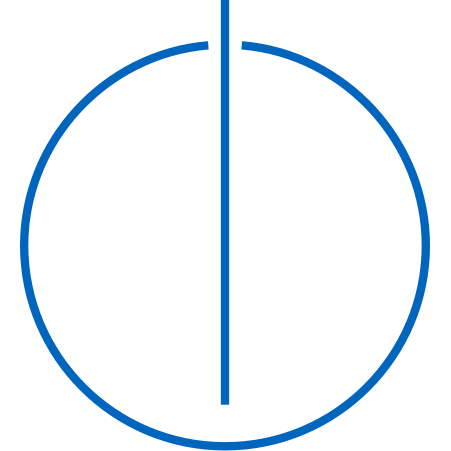
\includegraphics[height=20mm]{logos/faculty.png}
  }{}
\end{titlepage}

\cleardoublepage{}

\thispagestyle{empty}
\vspace*{0.8\textheight}
\noindent
\makeatletter
\ifthenelse{\pdf@strcmp{\languagename}{english}=0}
{I confirm that this \MakeLowercase{\getDoctype{}} is my own work and I have documented all sources and material used.}
{Ich versichere, dass ich diese \getDoctype{} selbstständig verfasst und nur die angegebenen Quellen und Hilfsmittel verwendet habe.}
\makeatother

\vspace{15mm}
\noindent
\getSubmissionLocation{}, \getSubmissionDate{} \hspace{50mm} \getAuthor{}

\cleardoublepage{}

\makeatletter
\ifthenelse{\pdf@strcmp{\languagename}{english}=0}
{\addcontentsline{toc}{chapter}{Acknowledgments}}
{\addcontentsline{toc}{chapter}{Danksagungen}}
\makeatother
\thispagestyle{empty}

\vspace*{20mm}

\begin{center}
\makeatletter
\ifthenelse{\pdf@strcmp{\languagename}{english}=0}
{\usekomafont{section} Acknowledgements}
{\usekomafont{section} Danksagungen}
\makeatother
\end{center}

\vspace{10mm}

%TODO: Acknowledgments
I would like to express my sincere gratitude to the BAC team at BMW for their invaluable support throughout my work. A very special thanks goes to my BMW supervisor, Johannes Urlhardt, for his tremendous guidance, support, and the generous time he dedicated to assist me. I am also deeply grateful to my university supervisor, Jianfeng Gu, for his understanding, advice, and continuous support during this project. Additionally, I would like to thank the company Vector for providing us with a license to use their software.

\cleardoublepage{}
 % TODO: if you don't have anyone to thank for or don't wish to publish it, comment this line out.
\chapter{\abstractname}

The automotive industry is rapidly transitioning toward software-defined vehicles, driven by the demand for enhanced convenience, safety, autonomy, and electrification. With millions of lines of code controlling various vehicle systems, ensuring their correct operation is critical \cite{synopsys2023software}. At BMW, the BMW AUTOSAR Core (BAC) serves as the foundation for deeply embedded ECUs, combining standardized AUTOSAR modules with BMW-specific extensions. However, traditional validation and testing methods for BAC software, which rely on physical hardware, are both costly and time-consuming. A complete test setup can cost between 2500 to 5000 Euros, limiting hardware access for many developers. This often results in delays and inefficiencies in the development process, as hardware issues or incorrect interpretations of requirements are discovered late.

This thesis addresses the challenges by implementing a fully virtualized test environment that eliminates the need for physical ECU hardware during the BAC software testing phase. Key challenges, such as replicating ECU behavior, enabling communication between the virtual ECU (vECU) and existing ECU testing tools, and accurately simulating the ECU’s modes, are tackled. Through this virtual environment, early-stage testing and debugging become possible, significantly accelerating the detection of software errors. Performance evaluations show that the virtual test setup can reliably simulate real-world conditions, offering developers a powerful tool for early and efficient testing.





%\makeatletter
%\ifthenelse{\pdf@strcmp{\languagename}{english}=0}
%{\renewcommand{\abstractname}{Kurzfassung}}
\renewcommand{\abstractname}{Abstract}
%\makeatother

%\chapter{\abstractname}

%TODO: Abstract in other language
%\begin{otherlanguage}{ngerman} % TODO: select other language, either ngerman or english !

%\end{otherlanguage}


% Undo the name switch
%\makeatletter
%\ifthenelse{\pdf@strcmp{\languagename}{english}=0}
%{\renewcommand{\abstractname}{Abstract}}
%{\renewcommand{\abstractname}{Kurzfassung}}
%\makeatother
\microtypesetup{protrusion=false}
\tableofcontents{}
\microtypesetup{protrusion=true}

\mainmatter{}

% !TeX root = ../main.tex
% Add the above to each chapter to make compiling the PDF easier in some editors.

\chapter{Introduction}\label{chapter:introduction}
%Use with pdfLaTeX and Biber.
In this chapter, we will define key terms essential for understanding the thesis topic. We will discuss the architecture of AUTOSAR and the ECU along with its various software parts. Finally, we will connect these concepts to outline the primary objective of the thesis and highlight my key contributions.

\section{The AUTOSAR software architecture}
The AUTOSAR (Automotive Open System Architecture) standard defines an architecture for embedded software on ECUs \cite{autosar2022}. AUTOSAR systems can be divided in four main components (see ~\autoref{fig:AUTOSAR}):
\begin{figure}[htpb]
  \centering
  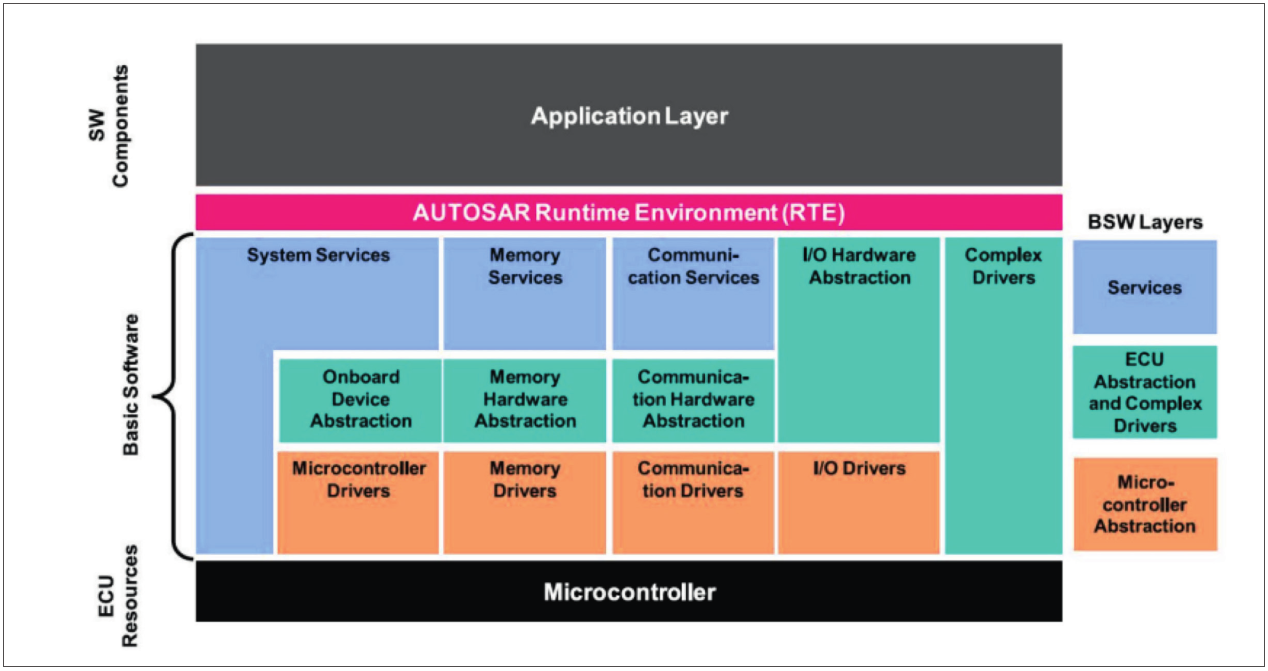
\includegraphics[width=1\textwidth]{figures/AUTOSAR}
  \caption{AUTOSAR (Classic Platform) ECU software layers \cite{smartse2020}.} \label{fig:AUTOSAR}
\end{figure}
\begin{enumerate}
\item \textbf{Application Software (ASW)} is the “highest layer” and comprises the control algorithm itself. This layer is called “Application Layer”. The content of this layer is, in most cases, the “system under test” (SUT). The BAC software components are located in this layer.
\item \textbf{Runtime Environment (RTE)} is the communication layer which distributes the signals directly between ASW components or using the base software’s (BSW) communication stack. The idea of AUTOSAR ASW components is that they can be distributed freely on different ECUs. The RTE will then either dispatch the data from one component directly to another component, if they are deployed on the same ECU, or the data is sent via the communication stack in the basic software.
\item \textbf{Basic Software (BSW)} is a software that provides a basic functionality of an ECU. The AUTOSAR Basic Software is further divided in the layers: Services, ECU Abstraction, Microcontroller Abstraction and Complex Drivers.
\begin{enumerate}
\item The Microcontroller Abstraction Layer (MCAL) is the lowest layer of the Basic Software. It manages access to the hardware, ensuring that high-level software does not directly interact with microcontroller registers. As a hardware-specific layer, MCAL provides a standardized interface for the basic software components, handling microcontroller peripherals and supplying them with hardware-independent values. MCAL also implements notification mechanisms to distribute commands, responses, and information across different processes. It can include components such as Digital I/O, Analog/Digital converters, Flash, and EEPROM.
\item The ECU Abstraction Layer interfaces the drivers of the Microcontroller Abstraction
Layer. It also contains drivers for external devices. It offers an API for access to peripherals and devices regardless of their location (µC internal/external) and their connection to the
µC (port pins, type of interface)
\item The Complex Drivers Layer spans from the hardware to the RTE, enabling direct access to Basic Software and/or hardware for resource-critical applications. It supports the integration of specialized functionality, such as drivers for devices not specified within AUTOSAR, those with strict timing constraints, or for migration purposes.
\item The Services Layer is the highest layer of the Basic Software. It provides essential functionalities, including operating system features, vehicle network communication and management services, memory services like NVRAM management, and diagnostic services such as UDS communication, error memory, and fault handling.
\end{enumerate}
\item \textbf{Microcontroller} is the actual hardware, which contains Internal devices, such as EEPROM, CAN controller, and ADC.
\end{enumerate}
\newpage
\begin{wrapfigure}{r}{0.4\textwidth}
  \centering
  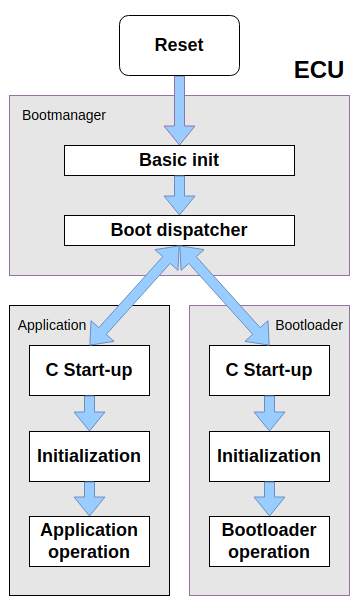
\includegraphics[width=0.9\linewidth]{figures/ECU.PNG}
  \caption{ECU Architecture.} \label{fig:ECU}
\end{wrapfigure}
\section{ECU Overall Architecture}\label{section:ECU_architecture}
Automotive ECUs typically contain three separate software parts, the Application, the bootmanager (BM), and the bootloader (BL).  After hardware or software reset of the ECU, the Bootmanager does certain basic initializations, and then jumps to the application or the bootloader. The bootmanager has no bus interface and no operating system. The Application implements the specific functionality of the ECU, e.g. controlling the engine or the airbags. The Bootloader allows to update the Application once the vehicle has been put on the market. ~\autoref{fig:ECU} provides an overview of the ECU overall architecture.

Although Application, Bootmanager and Bootloader are separate software parts, they require to exchange a minimum of information. This information is exchanged using a shared memory. After checking different conditions and flags, the bootmanager decides whether the Application or the Bootloader are started after a Reset. The Application is started, if there is no reprogramming request and the Application is valid. The Bootloader is started, if there is a reprogramming request or the Application is not valid. \cite{vectorBootloader} 

\section{Objective of the Thesis}
The main objective of this thesis is to develop a fully virtualized test environment tailored for the BMW AUTOSAR Core (BAC) software, enabling early software testing and more efficient debugging without relying on physical hardware. The virtualized environment is designed to replicate the functionality of a physical ECU using a virtual ECU and a virtual CAN bus. The goal is to enable ECU testing tools to interact with the vECU, send and receive CAN messages, and mimic the real ECU's behavior, including switching between various ECU modes.

\section{Thesis Contribution}
To create the virtual test setup, several missing components in the simulation needed to be developed. My primary contributions in this thesis include:
\begin{enumerate}
\item \textbf{Integrating the vECU into the test simulation}, enabling the testing of software components in a virtualized setup.
\item \textbf{Implementing an adapter} to facilitate communication between the vECU and the virtual CAN (vCAN) bus.
\item \textbf{Enabling data sharing between different ECU modes} to accurately represent real-world ECU behavior.
\item \textbf{Creating a unified simulation} that incorporates all ECU modes, allowing for accurate simulation of mode transitions, such as during resets or updates.
\item \textbf{Adjusting the timing} in the virtual environment to synchronize with real time, ensuring compatibility with testing tools that operate on a real-time basis, enabling accurate testing of the vECU.
\end{enumerate}

\section{Thesis Outline}
The structure of this thesis is organized as follows:
\begin{enumerate}
\item \textbf{Chapter 2} investigates state-of-the-art virtualization techniques and explores how similar projects use simulation, providing insight into different approaches.
\item \textbf{Chapter 3} compares traditional test setups with the virtual test setup implemented in this project. It introduces the software used in the virtual environment and the various testing tools employed.
\item \textbf{Chapter 4} details the core contributions of the thesis, focusing on the implementation of the adapter and the unified simulation. It provides an in-depth discussion of how these components were developed and integrated into the virtual environment.
\item \textbf{Chapter 5} discusses how virtual and real-time synchronization was achieved. It also presents the results of tests conducted on both the virtual and hardware setups, emphasizing the reliability of the virtual test environment in simulating real-world conditions.
\item The thesis concludes with a summary and a discussion of potential future work that could further enhance the virtual test environment.
\end{enumerate}
% !TeX root = ../main.tex

\chapter{Background}\label{chapter:Background}


This chapter explores the different levels of ECU virtualization, examining the advantages and disadvantages of each and identifying the most effective scenarios for their application. The latest virtualization techniques will be discussed, particularly their application in Real-Time Operating Systems (RTOS). Additionally, some promising software projects will be introduced as potential solutions for ECU virtualization in the case study. The goal of this chapter is to provide a solid understanding of the key concepts and tools essential for the thesis.

\section{vECU Classification}
The simulation of ECUs as virtual ECUs (vECUs) has quickly become integral in various stages of automotive development. Broadly, vECUs can be classified into two main categories: host compiled and target compiled \cite{synopsys2023software}.

Host compiled vECUs do not simulate the ECU hardware itself. Instead, they simulate Application Programming Interfaces (APIs) at key points in the software stack, effectively removing the need for lower, hardware-dependent layers. This means that the vECU does not run the complete production code, and certain layers must be modified. These modifications involve substituting specific software layers, not included in the system under test (SUT), with their simulated counterparts.

In contrast, target compiled vECUs use detailed hardware simulation models to accurately represent the ECU hardware. This enables the production software to run without requiring any alterations, as it is compiled exactly as it would be for the physical ECU used in a vehicle. To achieve this, detailed hardware modeling of the entire ECU is necessary, including its MCUs, internal CPU cores, components, and even board-level devices.

Dependent on the vECU content, different vECU levels can be distinguished. The following outlines an approach for defining and naming vECU layers \cite{smartse2020}, as depicted in ~\autoref{fig:levels}.
\begin{figure}[htpb]
  \centering
  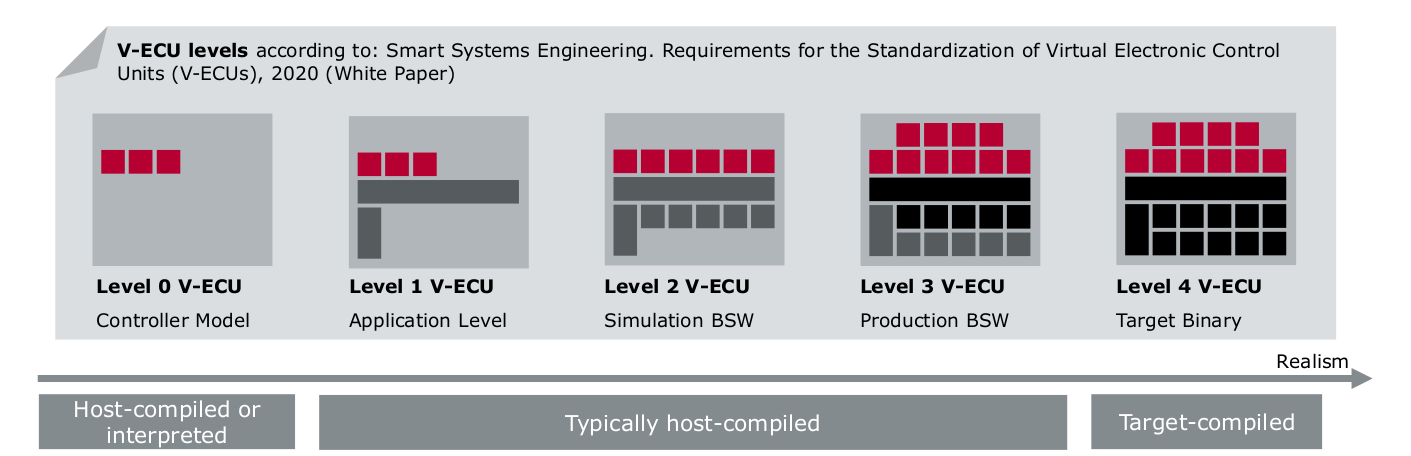
\includegraphics[width=1\textwidth]{figures/levels}
  \caption{Virtual ECU abstraction levels \cite{wenzler2023}.} \label{fig:levels}
\end{figure}

\subsection{Level 0}
The most basic form of ECU virtualization is the Level 0 vECU, which consists solely of the controller model. This model could be represented in various forms, such as a MATLAB Simulink model or C code derived from it. Importantly, this level of virtualization does not include any production code or basic software layers. As a result, Level 0 vECUs are limited to testing the control algorithms themselves and are not suitable for more comprehensive tests, such as software interface tests, which require more advanced types of vECUs closer to the actual production environment.

\subsection{Level 1}
Moving up in complexity, a Level 1 vECU includes the production code of the application software. However, to function correctly in a simulation environment, it requires additional functionalities from lower software layers. These supplementary layers are typically not from the production code but are specifically created or generated for the vECU. In AUTOSAR systems, for example, this would involve the Run-Time Environment (RTE) and the Operating System, along with other functionalities that enable the vECU to handle data transmission and reception. At this level, vECUs are primarily used for testing application functionalities, especially when these functionalities are distributed across multiple components or ECUs. However, they communicate only at the signal level and do not support bus or network communication.

\subsection{Level 2}
Level 2 V-ECUs add another layer of sophistication by incorporating simulated basic software (BSW) functionalities on top of the Level 1 components. Although these BSW functionalities are specifically created for simulation purposes and are not production-level, they enable more extensive testing capabilities. For instance, Level 2 vECUs can handle communication at the bus or network level, such as via simulated CAN or Ethernet, making them suitable for broader application software testing, including bus monitoring and diagnostic tests.

\subsection{Level 3}
At Level 3, vECUs include not only production application software but also production-level basic software (BSW), or in some cases, just the BSW or parts of it, depending on the testing requirements. The application and basic software at this level must be hardware-independent, such as everything above the microcontroller abstraction layer (MCAL) in AUTOSAR systems. While production BSW can be supplemented with simulated components for vECU purposes, the primary goal is to include as much of the real ECU's production code as possible. Level 3 vECUs are versatile, allowing for comprehensive testing of hardware-independent software, testing of networked vECUs, and even serving as rest bus models in hardware-in-the-loop (HIL) tests.

\subsection{Level 4}
The most advanced type of vECU, Level 4, includes the full production code compiled for the actual target ECU, including any hardware dependencies. This allows for a highly accurate simulation that mirrors the real ECU environment. To execute a Level 4 vECU on a simulation platform, an instruction set simulator is necessary, along with a detailed model of the ECU hardware. This level is particularly useful for testing scenarios that depend on the hardware architecture, such as evaluating the computational load of multicore ECUs. An example of level 4 vECU is the VDK from Synopsys \cite{synopsys_aurix_vdk_2020}. \\

To conclude, after evaluating the different levels of ECU virtualization, it becomes evident that Level 3 vECUs present the most suitable choice for implementation in this thesis. This level offers a balanced approach by including as much hardware-independent production code as possible without involving any physical hardware. By incorporating both the application software and the production basic software (BSW) while maintaining hardware independence, Level 3 vECUs allow for comprehensive testing and simulation. This makes them ideal for the scope of this research, where the focus is on maximizing software accuracy and functionality in a virtual environment.

\section{RTOS Simulation}\label{sec:RTOS}
When reviewing modern virtualization techniques, it is apparent that Real-Time Operating Systems (RTOS) virtualization shares many similarities with the level 3 virtualization discussed earlier.
This virtualization allows developers to run and test RTOS applications on a Linux environment, facilitating development and debugging processes without needing physical embedded hardware. Examples of RTOS platforms relevant to AUTOSAR standards include FreeRTOS, ThreadX, and Zephyr. These platforms are designed for applications that require precise timing and high reliability, making them suitable for use in automotive embedded systems.  
 
\subsection{Key Components of RTOS Simulation}
Several key components of an RTOS are emulated using the host OS features. These components include task management, the scheduler, interrupt handling, and timers.
\begin{enumerate}

\item \textbf{Task Management:} On actual hardware, tasks are managed using hardware-specific context-switching mechanisms. In simulation, tasks are represented as threads in the host OS, such as POSIX threads on Linux.

\item \textbf{Scheduler:} The scheduler in an RTOS is responsible for managing task priorities and context switching based on timing and event triggers. This functionality is emulated in software during simulation. The scheduler maintains the same logic for task prioritization and preemption, using host OS mechanisms to switch between threads.

\item \textbf{Interrupt Handling:} Hardware interrupts are critical in real-time systems for immediate response to events. These interrupts are serviced by specific interrupt service routines (ISRs). In a simulated environment, interrupts are emulated using host OS signals or inter-thread communication methods, creating handlers that mimic the behavior of ISRs.

\item \textbf{Timers:} RTOS relies heavily on hardware timers to trigger periodic tasks and manage timeouts. In simulation, host OS timers are used to replicate this functionality. For example, Linux system calls such as “setitimer” or “timer\_create” generate timer signals that simulate the periodic interrupts.
\end{enumerate}

\subsection{Simulation in Threadx}
ThreadX for Linux simulates an RTOS environment by utilizing POSIX pthreads to represent RTOS tasks and the scheduler. ~\autoref{fig:threads} gives an overview of the key implementation aspects \cite{threadx_readme}:
\begin{enumerate}
\item \textbf{Thread Representation: }
In the ThreadX simulation, each RTOS task is mapped to a POSIX pthread. When an application thread is created using the ThreadX API (e.g., tx\_thread\_create), a corresponding pthread is instantiated. These pthreads perform the same functions as their RTOS counterparts, allowing developers to test and debug real-time applications in a simulated environment.
\item \textbf{Scheduler Implementation: } 
The ThreadX scheduler is implemented as a high priority pthread. This scheduler thread determines which application thread to run based on their priorities and states. The scheduler preempts lower-priority threads to ensure that the highest-priority thread is always executing, mimicking the behavior of the RTOS on actual hardware.
\item \textbf{Simulated Interrupts: }
Simulated interrupts are handled using POSIX mechanisms such as signals. Interrupt Service Routines (ISRs) in ThreadX are mapped to signal handlers in Linux. When an interrupt is simulated, a signal is sent to the appropriate pthread, invoking the ISR. This allows the simulation to handle interrupts similarly to an actual RTOS.
\item \textbf{Timer Management: }
Timers in ThreadX are implemented using Linux system timers. Functions like "\textbf{setitimer}" or "\textbf{timer\_create}" generate periodic events, triggering timer-related tasks in the application. This ensures that timing behavior in the simulation is accurate and consistent with real-time requirements.
\end{enumerate}
\begin{figure}[htpb]
  \centering
  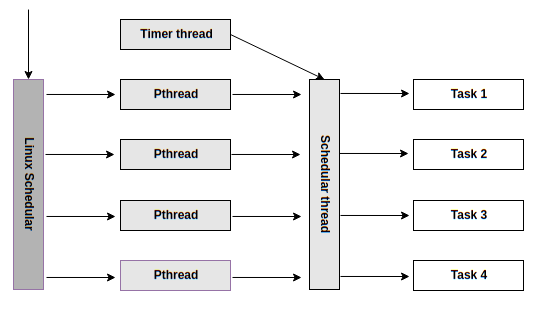
\includegraphics[width=0.8\textwidth]{figures/threads2}
  \caption{RTOS simulation on Linux.} \label{fig:threads}
\end{figure}


\subsection{Simulation in FreeRTOS}
The virtualization in FreeRTOS for Linux is achieved through a combination of Linux pthreads, mutexes, condition variables, and high-resolution timers. Here is a breakdown of how these elements are integrated \cite{freertos_simulator}:
\begin{enumerate}
\item \textbf{Pthreads for Task Management: }
Each FreeRTOS task is implemented as a pthread, allowing the FreeRTOS kernel to create, manage, and delete tasks in a manner analogous to its operation on embedded hardware.
\item \textbf{Condition Variables for Synchronization: }
FreeRTOS's synchronization primitives such as semaphores and queues are mapped to condition variables and mutexes in Linux. This mapping ensures that tasks can synchronize correctly even in a simulated environment.
\item \textbf{High-Resolution Timers for Tick Simulation: }
A dedicated high-priority thread generates periodic tick interrupts, simulating the hardware timer interrupts that FreeRTOS relies on. This thread sleeps for a specified interval (configurable to match the tick rate) and then signals the FreeRTOS scheduler to perform context switching and other periodic operations.
\item \textbf{Interfacing with Linux I/O: }
While the FreeRTOS simulator is running, it uses standard Linux system calls for I/O operations such as reading from and writing to the console. This makes it easier to debug and monitor the behavior of FreeRTOS tasks and system calls.
\end{enumerate}

\subsection{Simulation in Zephyr}
similar to ThreadX and FreeRTOS, Zephyr also provides a simulation environment that facilitates development and testing on host systems without the need for embedded hardware. This is achieved by virtualizing key components of the RTOS, leveraging the host operating system's features. Zephyr's simulation environment, particularly its native POSIX port, uses POSIX threads and system calls to emulate the behavior of the Zephyr kernel. \cite{zephyr_native_simulator}

\subsection{Benefits and Challenges of RTOS Simulation}
Simulation of RTOS offers several benefits. It is cost-effective as there is no need for physical hardware during the initial development phase. It is also flexible, allowing easy modification and testing of different configurations and scenarios. Additionally, it provides enhanced debugging capabilities using host OS tools, which can be more sophisticated than those available for embedded hardware.
While RTOS simulation provides a valuable platform for development and testing, it is important to acknowledge its limitations:
\begin{enumerate}
\item \textbf{Non-Real-Time Behavior: } The simulator runs on a general-purpose Linux operating system, which does not guarantee real-time behavior. Therefore, timing accuracy and real-time performance cannot be ensured.
\item \textbf{System Call Overheads: } Console I/O and other Linux system calls can interfere with the RTOS simulation, potentially affecting task execution and timing.
\item \textbf{Hardware-Specific Features: } Certain hardware-specific features and peripherals cannot be accurately emulated in the simulation environment.
\end{enumerate}
% !TeX root = ../main.tex

\chapter{From Traditional Hardware Setup to Virtual Setup}\label{chapter:simulation}
In this chapter, we explore the transition from a traditional hardware-based test setup to a fully virtualized test environment. We examine the components of a typical hardware test setup and identify what needs to be replaced or adapted to achieve a comprehensive virtual test system. The chapter also delves into the key tools utilized for simulating and testing vECUs within the scope of this thesis. These tools, including vVIRTUALtarget, Vector SIL Kit, and the Vector XL Library, are essential for creating a seamless and efficient virtual ECU development environment.


\section{The Traditional Test Setup}
The traditional test setup involves a computer running "ECU-TEST", which is connected to a "Vector hardware interface". This interface is then linked to an evaluation board via a system bus, such as CAN, FLEXRAY, or Ethernet (ETH). Additionally, a power supply is included in the setup to control the power to the ECU, allowing for power cycling and hardware resets. \autoref{fig:hardware_test_setup} illustrates the traditional test setup, highlighting the presence of the physical ECU within the testing environment. \autoref{fig:Real_hardware} shows the picture of an actual evalboard.



\begin{figure}[htpb]
  \centering
  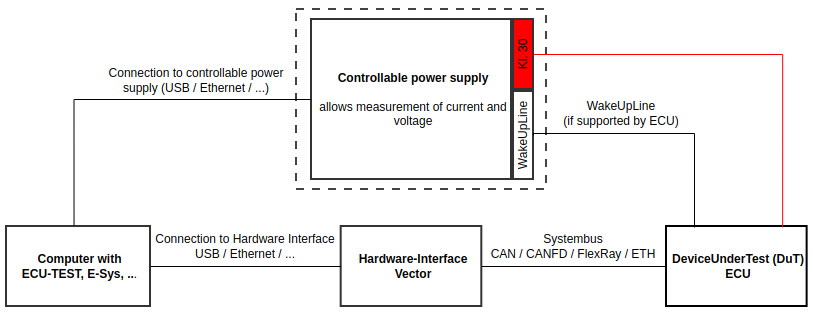
\includegraphics[width=1\textwidth]{figures/Hardware_setup.PNG}
  \caption{Sketch of a traditional test setup with an actual ECU.} \label{fig:hardware_test_setup}
\end{figure}

\begin{figure}[htpb]
  \centering
  \rotatebox{0}{ % Rotate the image by 90 degrees
    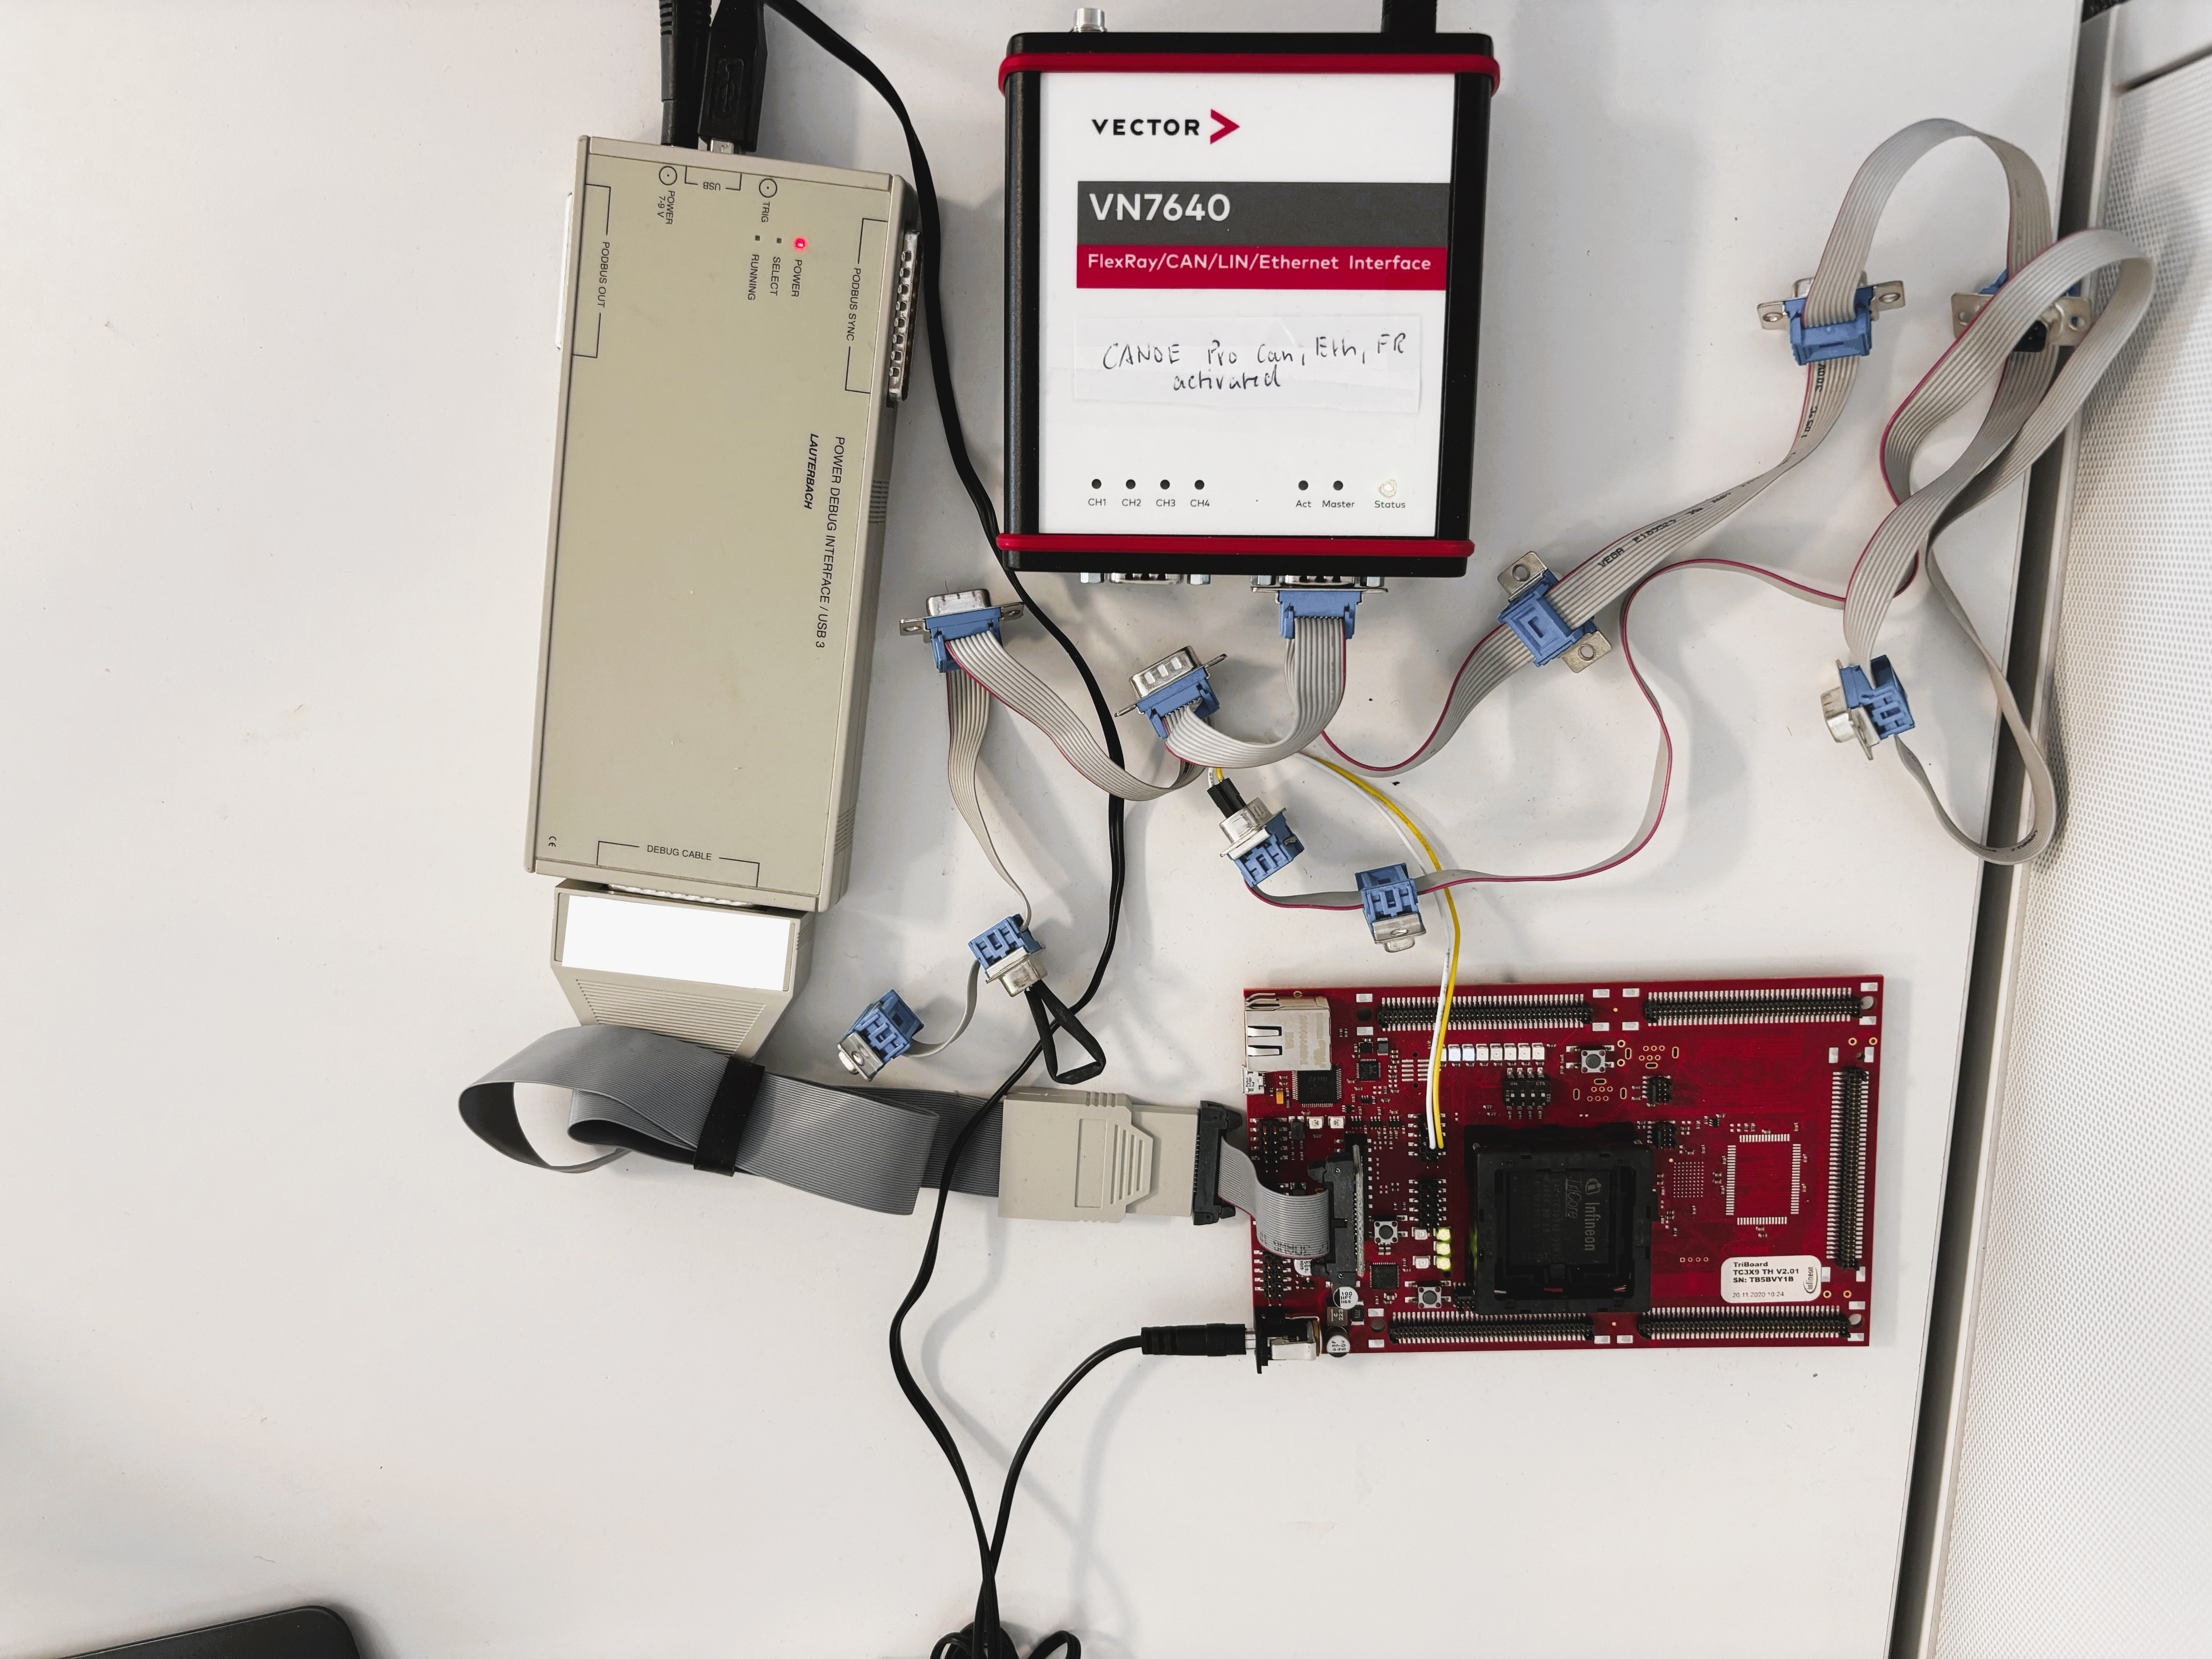
\includegraphics[width=0.65\textwidth]{figures/Real_hardware.jpg}
  }
  \caption{Real image of an ECU test setup.} 
  \label{fig:Real_hardware}
\end{figure}





\section{The Virtual Test Setup}
The objective of the virtual test setup is to replicate the functionality of the traditional hardware setup without the need for physical hardware. To achieve this, the real CAN bus is replaced with a virtual CAN bus (vCAN), as the test tools are already compatible with this interface. Next, the Vector hardware interface is substituted with "SIL KIT", which is a software capable of integrating the virtual ECU (vECU) into the simulation environment. Additionally, an adapter is required to facilitate the transmission of CAN messages between the vCAN and the vECU. \autoref{fig:test_setup} depicts the fully virtualized test setup implemented to replace the traditional hardware configuration. A detailed explanation and description of this implementation will be provided in the subsequent chapters.


\begin{figure}[htpb]
  \centering
  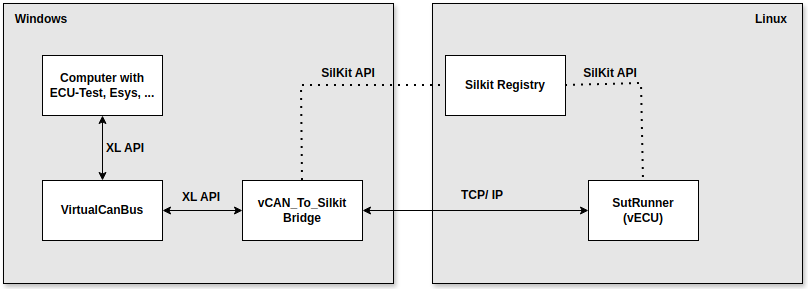
\includegraphics[width=0.97\textwidth]{figures/test_setup2.PNG}
  \caption{vECU test setup.} \label{fig:test_setup}
\end{figure}


\section{Simulation Host Environment}
As depicted in \autoref{fig:test_setup}, the testing simulation environment is divided between Linux and Windows platforms. This split is due to the current development and testing infrastructure. All BAC software development primarily takes place on Linux, and the Continuous Integration (CI) systems are also predominantly Linux-based. Running tests and executing processes on Linux is more efficient, largely due to the advantages Linux offers, such as containerization, which simplifies the CI workflow.





On the other hand, tools like ECU-Test and Esys are traditionally Windows-based. While there is a Linux version of Esys, it is limited to command-line functionality. Although the long-term plan is to move entirely to Linux, for now, Windows is still required for certain aspects of the testing process.

While it is technically possible to run the entire SIL Kit simulation on Windows and compile the source code there, this approach doesn't align with the broader strategy of maintaining a Linux-centric development and testing environment. The emphasis on containerization in the CI pipeline—especially in environments like AWS and on BMW’s servers—makes Linux the preferred choice, as Windows lacks the robust container support that Linux provides.

\section{vVIRTUALtarget}
vVIRTUALtarget is an innovative tool that allows for the simulation and testing of ECU software without needing real target hardware. It achieves this by providing virtualized OS and MCAL (Microcontroller Abstraction Layer) modules, which are essential for running the virtual ECUs generated by vVIRTUALtarget in custom environments. The virtualization technique used is very similar to that discussed in \autoref{sec:RTOS} for RTOS virtualization. ~\autoref{fig:vVirtualTarget} shows where the vVIRTUALtarget modules are located in the AUTOSAR architecture. \cite{vector_vvirtualtarget}

\begin{figure}[htpb]
  \centering
  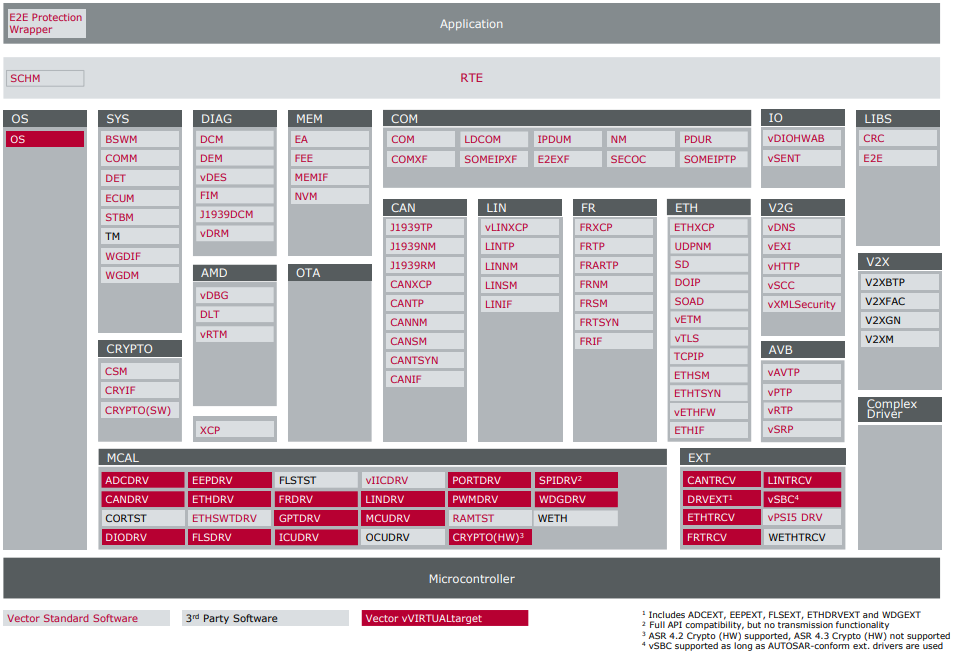
\includegraphics[width=0.83\textwidth]{figures/vVirtualTarget.PNG}
  \caption{vVIRTUALtarget virtualized layers In The 
AUTOSAR architecture \cite{user_man}.} \label{fig:vVirtualTarget}
\end{figure}

The tool is versatile, supporting various build systems, compilers, and development environments, including CMake, Microsoft Visual Studio, and MinGW-w64. Essentially, the virtual ECU generated by vVIRTUALtarget is a Windows Dynamic Link Library (DLL) or a Linux shared object (.so) file, which can be integrated with other testing tools using the OpenSUT programming interface.

The process of generating a virtual ECU involves using DaVinci Configurator Classic to configure, validate, and generate the basic software (BSW) and runtime environment (RTE) of an AUTOSAR Classic ECU. Once the project is validated and the code is generated, the project file (.vttproj) can be opened in vVIRTUALtarget. The tool then generates a Microsoft Visual Studio solution for windows or a Cmake file for linux, to create a DLL/SO for the virtual ECU.

Key configuration steps include defining application source files to be included in the solution. The tool automatically generates several files, such as:
\begin{enumerate}
\item \textbf{CANoeEmu\_cfg.c: } A source file containing handler functions for the runtime library.
\item \textbf{Vtt\_Hook.c and Vtt\_Hook.h: }Provide hook and handler functions for vVIRTUALtarget.
\end{enumerate}

vVIRTUALtarget not only generates a virtual ECU but also creates a standalone System Under Test (SUT) executable, enabling out-of-the-box connectivity with the Vector SIL Kit. When running as a standalone SUT, the virtual ECU operates as a separate process and can interact with tools like CANoe via the Vector SIL Kit, leveraging the OpenSUT API for flexible integration into a custom environment. \cite{user_man}

\subsection{Structure of the Shared Object Simulation}\label{subsec:structure_of_simulation}
Within the shared object, there is a directory named "\textbf{CanoeEmu}", which houses both header and source files essential for the simulation process. This directory includes key files such as "\textbf{CANoeEmuLibExport.h}", which is responsible for exporting functions from the "\textbf{libcanoe}" library, and "\textbf{CANoeEmu\_DllMain.cpp}", which provides the necessary functions to be exported from the VTT SUT Library. Additionally, "\textbf{CANoeApi.h}" contains prototypes for the CANoe APIs used throughout the simulation.

During the build process, the "\textbf{CanoeEmu}" directory is linked with the "\textbf{libcanoe}" library within the \textbf{CMake} configuration, ensuring that all required dependencies are in place. When the SUTRunner executable loads the shared object, several functions from the "\textbf{CanoeEmu}" directory are dynamically loaded and invoked at runtime. These functions play a critical role in initializing data, locating the main function within the shared object, and simulating various hardware behaviors.

The first function called upon loading the shared object is "\textbf{opensut\_init}", which is responsible for initializing the SUT. This function, in turn, calls an essential function named "\textbf{CANoeAPI\_InitHook}". The "\textbf{CANoeAPI\_InitHook}" must be implemented by any application utilizing the CANoe emulation library, as it serves as the central initialization hook for the emulation. Within this initialization hook, various init functions can be used to configure multiple aspects of the emulation, ensuring that the system is properly set up for accurate simulation.

\section{Vector SIL Kit}
Vector SIL Kit (Software-in-the-Loop Kit) is a versatile tool designed for simulating, testing, and validating distributed automotive systems, particularly focusing on environments with virtual ECUs. SIL Kit enables co-simulation, allowing multiple ECUs and other system components to interact within a unified simulation environment. This removes the need for physical hardware during testing, making it especially useful in early development stages. SIL Kit supports complex automotive testing scenarios, including system interactions, timing, and performance analysis, using simulated networks such as CAN or Ethernet, replicating the communication in real vehicle systems. \cite{sil_kit_github}

\subsection{How SIL Kit Works}
A SIL Kit simulation setup consists of several key components: the \textbf{SIL Kit Registry} and one or more simulation \textbf{participants} (e.g., virtual ECUs). The \textbf{SIL Kit Registry} plays a central role, as it is responsible for connecting and managing communication between all participants. The registry must be started before any participants are created, acting as a broker that enables discovery and connection between participants.

Here’s a breakdown of the SIL Kit process \cite{sil_kit_docs}:

\begin{enumerate}
\item \textbf{Registry: } The SIL Kit Registry is the first component that must be launched. It listens for participants on a specified URI and provides connection information, allowing participants to establish peer-to-peer connections.
\item \textbf{Participants: } Each participant, whether it's a virtual ECU or another software component, connects to the registry to obtain information about other active participants. Once the connection information is exchanged, participants communicate directly, forming a simulation network. SIL Kit supports network types like TCP/IP and Unix Domain Sockets to facilitate these connections.
\item \textbf{Simulation Setup: } When a new participant joins, it opens a public listening socket and connects to the registry. The registry then provides the participant with the connection details of other participants, enabling direct peer-to-peer communication. By default, participants attempt to connect via Unix Domain Sockets and fall back on TCP if necessary.
\item \textbf{Simulation Task: } The actual simulation happens through a callback mechanism, which is triggered as simulation time progresses. This is done using the time synchronization service by registering the \textbf{SetSimulationStepHandler()} callback. 
\end{enumerate}

\begin{figure}[htpb]
  \centering
  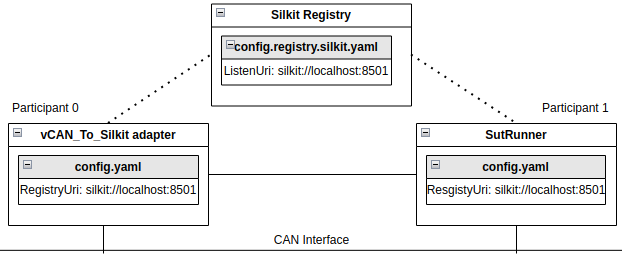
\includegraphics[width=0.83\textwidth]{figures/silkit_connection.PNG}
  \caption{ Simulation setup with two participants that communicate on a CAN bus network.} \label{fig:silkit_conn}
\end{figure}

\subsection{Integration with vVIRTUALtarget}
In this project, SIL Kit integrates seamlessly with vVIRTUALtarget. The SutRunner generated by vVIRTUALtarget is connected to the SIL Kit environment as a participant in the simulation. Additionally, an adapter is developed and connected to SIL Kit as a separate participant.

As shown in \autoref{fig:silkit_conn}, the two participants— the SutRunner and the adapter— exchange their connection information through the SIL Kit Registry, enabling smooth communication over a simulated network. This setup ensures that the vECU and the testing tools can interact within a cohesive simulation, mimicking real-world conditions for early testing and debugging.

\subsection{Time Synchronization in SIL Kit}
When the \textbf{TimeSyncService} is used in SIL Kit, participants follow a synchronized virtual time framework, ensuring that each component in the distributed simulation advances in lockstep with the others. The service allows for configuring the size of each simulation step and setting up handlers that get called at each step. As the virtual time progresses, the step handler is triggered to allow the participant to carry out its tasks at that moment. SIL Kit guarantees that the virtual time moves forward consistently—without skipping or repeating any steps—according to the configured interval for each participant. \cite{sil_kit_docs}

\subsubsection{Autonomous vs. Coordinated Modes}
SIL Kit offers two modes of operation for participants: \textbf{Autonomous} and \textbf{Coordinated}. When running in \textbf{Coordinated} mode, participants synchronize their states, ensuring that all essential components are aligned before beginning the simulation. This coordinated setup is necessary when multiple participants need to reach the Running state simultaneously, as the simulation will only start once all participants are ready. If one participant calls Stop(), the entire group of coordinated participants will pause, making this mode suitable for tightly synchronized environments where collective actions are essential.

On the other hand, in \textbf{Autonomous} mode, each participant runs independently of the others. In this mode, participants don’t wait for synchronization, and each can start and stop its simulation without affecting the others. This is ideal for situations where timing synchronization is unnecessary across participants, allowing for more flexibility.

\subsubsection{Synchronization Between the vECU and the Adapter}
In this project, \textbf{vVIRTUALtarget} originally used Coordinated mode for the \textbf{SutRunner}, expecting the vECU to synchronize with other virtual ECUs in the system. However, since the \textbf{ECU-Test} tool operates in real time, it wouldn’t make sense to coordinate the adapter with the virtual time, as the adapter’s role is simply to forward CAN messages as they arrive. Coordinating the adapter would only make sense if ECU-Test was also working with virtual time, which it isn’t.

Because of this, the \textbf{SutRunner} was switched to \textbf{Autonomous mode}, allowing it to function independently. In this setup, the adapter forwards messages in real time, and the simulation doesn’t require strict synchronization with the vECU. This adjustment ensures that the real-time nature of ECU-Test is maintained, while still leveraging the benefits of the virtual environment.

\section{Vector XL Library}
The Vector XL Library is another essential tool that will be utilized in this project. It provides a comprehensive set of functions and APIs for interacting with Vector's hardware and software products, facilitating communication and data exchange within automotive networks.

The XL Library abstracts the complexities of hardware communication, allowing developers to interact with various bus systems such as CAN, LIN, FlexRay, and Ethernet using a consistent API. This abstraction simplifies the development process and ensures compatibility across different hardware setups.

The Vector Hardware Config tool is required to set up the hardware settings like virtual channel assignment etc. The management of the application settings can be either done in the tool or via get/set functions of the XL Driver Library. \cite{xl_driver_library_manual}

\section{Software tools for testing}
In the context of BMW vehicles, there are multiple software tools used for testing and validating the ECUs, such as AmTS and Esys.

The development, testing, and validation of vehicle software and hardware components, including Electronic Control Units (ECUs), within BMW vehicles are facilitated by a comprehensive quality assurance technology stack known as the Automotive Test Suite (AmTS) \cite{automotive_test_suite_2022}. This system serves as the foundation for a streamlined and automated testing process, where relevant test plans are implemented in the "\textbf{ECU-TEST}" automation tool and executed automatically for each ECU. The test results are then seamlessly integrated into the "\textbf{TEST-GUIDE}" test report management system, providing clear and accessible data for all stakeholders involved.

\textbf{Esys} is another specialized software tool that is widely utilized by BMW engineers to code, program, and configure the ECUs in BMW vehicles. This software tool plays a vital role in the overall process of ensuring the proper functioning and integration of the vehicle's electronic systems.


\section{Unified Diagnostic Services (UDS)}
The Unified Diagnostic Services (UDS) protocol is a key communication system used in automotive diagnostics \cite{iso_14229}. It enables diagnostic tools to interact with an ECU by sending requests and receiving responses, much like how diagnostic communication works on physical cars. The UDS protocol can be understood as a communication method between a testing tool and the ECU in vehicles, somewhat analogous to HTTP requests used on the web. Both UDS and HTTP requests follow a request-response model, but they operate in different contexts.

UDS operates on the CAN bus and is used for various tasks such as fault diagnosis, reading sensor data, and flashing firmware. Through standardized services, UDS allows for complex operations such as software updates, troubleshooting, and testing the behavior of ECUs by sending specific commands. These commands use service identifiers (SIDs), like the commonly used 0x22 for "Read Data by Identifier" to extract system data\cite{uds_tutorial}.

In the context of testing virtual ECUs (vECUs), UDS messages are essential because they simulate the same interactions a real-world ECU would encounter. By sending UDS requests over a virtual CAN (vCAN) bus, we can validate whether the vECU behaves as expected, ensuring it is capable of handling real-world diagnostic operations. This process is crucial during testing phases to ensure the system's accuracy before physical deployment.\\


In conclusion, the combination of vVIRTUALtarget, Vector SIL Kit, and the Vector XL Library forms a comprehensive ecosystem for the simulation, testing, and validation of virtual ECUs. These tools enable the development of sophisticated and reliable automotive software, allowing for thorough testing in both virtual and hybrid environments. However, some adaptations are still needed to achieve a fully virtual test setup.
% !TeX root = ../main.tex
% Add the above to each chapter to make compiling the PDF easier in some editors.

\chapter{Implementation of vECU Setup}\label{chapter:Implementation}
In this chapter, we explore the practical implementation of the vECU setup as part of this thesis. The chapter provides a comprehensive and detailed account of each step involved in the process, ensuring a clear understanding of how the virtual ECU environment was constructed. It not only covers the technical aspects of the setup but also delves into the various challenges and complexities encountered along the way. Additionally, the chapter discusses the different strategies and solutions that were considered to overcome these obstacles, offering insights into the decision-making process. Finally, it outlines the rationale behind the final approach that was chosen, explaining why it was deemed the most effective solution for achieving the project’s goals.

\section{vCAN to SilKit Adapter}
After successfully building the application component of the vECU as a shared object in Linux using vVirtualTarget and establishing a connection between the SUTRunner and the SIL Kit registry, as discussed in the previous chapter, the next major challenge was to facilitate seamless communication between the vECU and external testing tools. This was particularly challenging because most of the testing software used at BMW, such as ECU-test \cite{ecu_test} and Esys, operates on Windows and relies on sending and receiving UDS requests and responses via a CAN bus to interact with the ECU. To bridge this communication gap, a specialized adapter called the "\textbf{vCAN\_To\_SILKit}" adapter was developed, which connects the virtual CAN bus to the SIL Kit registry, enabling smooth communication. ~\autoref{fig:test_setup} provides a visual representation of the entire test environment, highlighting the role of the adapter.

The "\textbf{vCAN\_To\_SILKit}" adapter is a crucial tool designed to  facilitate the interaction between the vECU and the testing software. The process to set up this adapter involves several key steps:


\begin{enumerate}
\item \textbf{Setting up the Virtual CAN Interface}: A virtual CAN interface is first configured on the Windows system using the Vector Hardware Configuration tool.
\item \textbf{Launching the "vCAN\_To\_SILKit" Adapter}: The adapter is then launched, binding to the virtual CAN interface on one side via the xlAPI interface, while on the other side, it connects to the SIL Kit as a participant in the simulation environment.
\item \textbf{Connecting SUTRunner to SIL Kit}: Once the adapter is operational, the SUTRunner software is started, and its connection to the SIL Kit registry is established, ensuring that all components are in sync.
\item \textbf{Running ECU-test}: With all connections successfully in place, the ECU-test software can be executed to transmit and receive CAN messages to and from the vECU through the "\textbf{vCAN\_To\_SILKit}" adapter, enabling comprehensive testing and validation of the vECU setup.
\end{enumerate}

This setup allows the ECU-test to interact with the virtual CAN interface, which is then bridged to the SIL Kit CAN bus, enabling testing and validation of the ECU without the need for physical hardware.

\subsection{Adapter to silkit}
The initial step in connecting the adapter to the SIL Kit registry involves creating a simulation participant. This is achieved using the "\textbf{SilKit::CreateParticipant}" function, where the participant is named "\textbf{vCAN\_To\_SILKit\_Adapter}", and both the "\textbf{registryUri}" and participant configuration are specified.

Once the "\textbf{IParticipant}" is established, a lifecycle service is created to manage the workflow and state transitions of this simulation participant. The lifecycle service is essential as it provides access to the time synchronization service, allows for the registration of callbacks for state changes, queries the participant’s current state, and issues commands to transition between states.

With the "\textbf{IParticipant}" instance in place, various SIL Kit services can be created and accessed. One of the critical services for this adapter is the CAN Service API, which offers a CAN bus abstraction via the "\textbf{ICanController}" interface. The CAN controller is instantiated by calling "\textbf{CreateCanController}", where the controller and network names are provided.

This "\textbf{ICanController}" is then passed as an argument to the "\textbf{create}" function, which is responsible for establishing the connection with the virtual CAN (vCAN) side. Once the setup is complete, the simulation can be initiated using the "\textbf{StartLifecycle}" method, which runs the simulation until it is either stopped or aborted. \cite{sil_kit_docs}


\subsection{CAN connection implementation}
This subsection provides a comprehensive overview of the process involved in implementing the connection to the virtual CAN (vCAN) network. 

At the heart of this connection lies the "ClassicalCanConnectionImpl" struct, which serves as the core component responsible for handling the intricate details of CAN message management. This struct is designed to effectively control the flow of CAN messages, ensuring they are accurately transmitted from the vCAN network to the SIL Kit network and vice versa. 

In ~\autoref{lst:can_connection}, the definition of the ClassicalCanConnectionImpl struct is presented. The listing not only outlines the structure of the implementation but also provides insights into how each function within the struct contributes to the overall process of CAN message management. 

\newpage

\begin{lstlisting}[caption={The ClassicalCanConnectionImpl struct.}, label={lst:can_connection}]
struct ClassicalCanConnectionImpl
{
public:
    ClassicalCanConnectionImpl() = default;
    ~ClassicalCanConnectionImpl() = default;

    //converts the CAN message from XLevent to a silkit CAN frame 
    CanFrame XLTOSILKIT(XLevent* event);

    // Writes the SIL Kit CanFrame to the vCAN
    void WriteToXL(XLportHandle portHandle, XLaccess accessMask, const CanFrame& SilkitFrame);

    // Handles received frames from the vCAN and sends them on the SIL Kit 
    void HandleReceivedCanFrameFromVirtualCanDevice(ICanController* canController,SilKit::Services::Logging::ILogger* logger, XLevent* event);

private:
    // Temporarily stores the CAN frame that is to be sent to the vCAN device
    XLevent _frameToVCAN;
};
\end{lstlisting}

\subsection{Adapter to vCAN}
  
This subsection delves into the other crucial aspect of the adapter: the connection to the virtual CAN (vCAN) network via the XL API. The integration between the SIL Kit API and the XL API begins with the create function, where the foundational connection is established. Within this function, an instance of the "\textbf{ClassicalCanConnectionImpl}" struct is created to manage the communication process.

The first step in this process is to initialize a virtual CAN connection. This involves several critical actions: opening an XL driver, retrieving the application configuration, opening the necessary port, and finally, activating the channel. These steps ensure that the vCAN is ready to transmit and receive CAN messages. \cite{xl_driver_library_manual}

On the transmission side, sending CAN messages from the SIL Kit to the vCAN is handled by the WriteToXL function within the "\textbf{ClassicalCanConnectionImpl}" struct. This function is linked to the SIL Kit by passing it to the AddFrameHandler function within the "\textbf{ICanController}", facilitating smooth communication between the two APIs.

For receiving messages, the process is managed by the ReceiveThread function, which operates in a continuous loop on a separate thread. This thread listens for incoming CAN messages using the xlReceive function. Upon receiving a message, it invokes the "\textbf{HandleReceivedCanFrameFromVirtualCanDevice}" function within the "\textbf{ICanController}", ensuring that messages are efficiently transferred from the vCAN to the SIL Kit network.

\subsection{Optimizations within the adapter}
To enhance the efficiency of CAN message transmission through the adapter, several key optimizations were implemented. These optimizations focused on reducing overhead and improving the speed of data transfer.

One significant optimization involved disabling receipt acknowledgments when a message is transmitted or when it is queued for transmission. By eliminating these acknowledgments, the system reduces unnecessary overhead, thereby accelerating the message transfer process.

Another critical optimization was applied to the receive thread. Originally, this thread continuously ran in an infinite loop, constantly checking for incoming messages. To eliminate the inefficiency of busy waiting, the thread was modified to wait for notifications from the receive queue. This was achieved using the "\textbf{xlSetNotification}" function, which configures the queue level for notifications on the specified port and returns a notification handle. This handle, linked to an auto-resetting Windows event, remains valid until the port is closed. By relying on event-driven notifications rather than constant polling, this approach significantly reduces CPU usage and enhances the overall performance of the adapter.

\section{A Unified Virtual Simulation}
In \autoref{section:ECU_architecture}, we discussed the three distinct software components of the ECU: the Application, the Boot Manager (BM), and the Bootloader (BL). A significant challenge in this project was the inability to virtualize these components as a single entity due to the limitations of our available software, which only allows for the virtualization of each software part separately. As a result, each component operates as an independent shared object within its own isolated simulation.

This separation presented a major obstacle, as it prevented the seamless integration and interaction of these components, which is essential for realistic testing and validation. In a physical ECU, the Boot Manager typically initializes some shared data, and controls the flow between the Application and the Bootloader, making it crucial for the virtual environment to replicate this behavior \cite{embeddedartistry_before_main}. Therefore, a unified simulation environment needed to be developed, one that could integrate all three software parts into a single cohesive simulation. This environment would not only have to manage the shared resources among the different components but also enable the Boot Manager to dynamically control which main function—whether the Application or the Bootloader—should be executed.

This section provides a detailed account of these approaches, discussing the various options that were considered, the reasoning behind each, and the iterative process that led to the final solution. \autoref{fig:vECU_setup} shows the desired vECU setup that can simulate the behavior of the actual ECU. 

\begin{figure}[htpb]
  \centering
  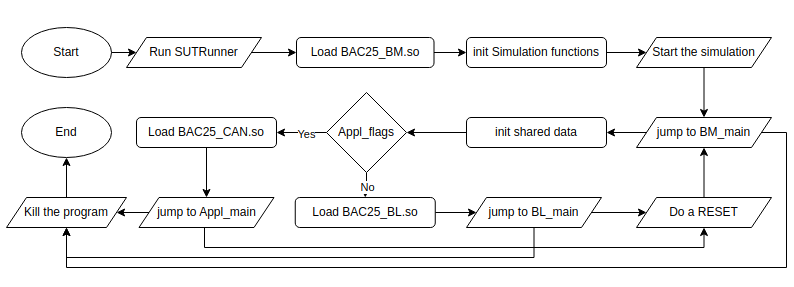
\includegraphics[width=1\textwidth]{figures/complete_setup.PNG}
  \caption{Interaction between the Application, BL, and Bm indise the vECU.} \label{fig:vECU_setup}
\end{figure}

\subsection{Initial Concept: Sequential Simulation Switching}
When initially considering how to manage the transition between the different software components of the ECU—the Application, Boot Manager (BM), and Bootloader (BL)—one approach that seemed straightforward was to handle these transitions by sequentially stopping and starting separate simulations. For example, once the Boot Manager completed its task, the idea was to halt its simulation and then initiate the simulation for the Application, and so forth.

At first glance, this approach appeared to offer a simple solution for managing the distinct phases of the ECU’s operation. However, upon deeper analysis, several critical flaws became evident. The most significant issue was the lack of shared data between the separate simulations. In a real ECU, these software components must communicate seamlessly, sharing state information and other critical data. This communication is essential for the system’s overall functionality, especially when transitioning between modes, such as from the Boot Manager to the Application or vice versa.

Without a mechanism to share data, each simulation would operate in isolation, leading to a disjointed system where no actual communication occurs between the components. This isolation not only disrupts the flow of information but also hinders the accurate replication of the ECU’s behavior during mode transitions. Furthermore, this approach made it impossible to emulate critical ECU behaviors, such as resetting and returning control to the Boot Manager to determine the next action. In a real-world scenario, such transitions are fluid and interconnected, something this approach could not replicate.

Given these limitations and the need for a more integrated and realistic simulation environment, the idea of running three separate simulations was ultimately deemed unworkable. It became clear that a unified simulation, where all components could interact within a single, cohesive environment, was essential to accurately emulate the ECU’s behavior and ensure that the software components could function together as they would in an actual ECU system.
\newpage
\subsection{Sharing Data Among Shared Objects}
Given that the three software components—the Application, Boot Manager (BM), and Bootloader (BL)—are each represented as shared objects, the challenge of sharing data among them had to be addressed. These shared objects are dynamically loaded within the SUTRunner executable, and two primary approaches for data sharing were considered.

The first approach involved defining a common memory section within the SUTRunner. This memory would be shared across the different shared objects by using "\textbf{memcpy}" to transfer data from the common memory to the local memory of a specific shared object before each function call. After the function execution, the data would then be copied back to the common memory. While this method could technically facilitate data sharing, it introduced significant drawbacks. The constant memory transfers would lead to unnecessary delays and increased memory usage, both of which are undesirable in a performance-sensitive environment. Consequently, this approach was deemed inefficient.

The second, more efficient approach leverages the dynamic loading capabilities provided by the "\textbf{dlopen}" function. In this method, all three shared objects are loaded dynamically, with the Boot Manager being loaded first and with the "\textbf{RTLD\_GLOBAL}" flag. This flag ensures that the symbols defined by the Boot Manager are made globally available for the resolution of symbols in the subsequently loaded shared objects \cite{dlopen_man_page}. As a result, the Boot Manager's data becomes accessible to the Application and Bootloader, allowing for seamless data sharing among the three components without the need for costly memory copying operations. This approach not only simplifies the data-sharing process but also enhances the overall efficiency of the system.

\subsection{Unified Simulation Approach}
After successfully establishing a method to share data among the three shared objects, the next significant challenge was to consolidate the three separate simulations into a single, unified simulation. The structure of a single simulation has already been discussed in \autoref{subsec:structure_of_simulation}.

To achieve a unified simulation, the first step was to extract the "\textbf{CanoeEmu}" directory from each of the shared objects, along with the "\textbf{libcanoe}" library,  and build this as a standalone shared object. This new shared object could then be linked to the three other shared objects, enabling them to utilize the same "\textbf{libcanoe}" library and share the same initialization functions and resources. However, this approach introduced new challenges during the linking process.

One of the challenges encountered was the inability to locate certain function definitions that were previously exported directly to the shared objects from the "\textbf{libcanoe}" library when linked within the CMake files. To resolve this, function prototypes were included within the "\textbf{CanoeEmu}" shared object. These prototypes act as intermediaries, making the "\textbf{libcanoe}" functions accessible to the other shared objects. Each prototype has the same signature as its corresponding function in the "\textbf{libcanoe}" library and simply forwards calls to the actual function. An example of such a prototype is shown in ~\autoref{lst:SetMain}.
\newpage
\begin{lstlisting}[caption={SetMainFunction Prototype.}, label={lst:SetMain}]
extern "C"  
void CANoeAPI_SetMainFunction_caller(void(*main)(void))
{
  CANoeAPI_SetMainFunction(main);
}
\end{lstlisting}

Another challenge involved the initialization of certain data that was previously handled within the application but not within the boot manager. Since only the boot manager’s initialization function is called in this setup, it was necessary to find a way to ensure that all required data was properly initialized within the boot manager.

A critical function, "\textbf{CANoeAPI\_OnStateChange}", which is responsible for handling global state changes in "\textbf{CanoeEmu}", was only initialized within the application shared object. This function propagates state changes to the configured modules, and without its initialization in the application, the simulation would encounter errors and enter an infinite loop.

To address this, the "\textbf{CANoeAPI\_OnStateChange}" function within the boot manager was redefined as a prototype that references the same function in the application shared object. By loading the function from the application shared object and calling it within the boot manager, we ensured that initialization in one shared object would impact all shared objects. An example of how this can be implemented is shown in ~\autoref{lst:StateChange}.


\begin{lstlisting}[caption={Calling CANoeAPI\_OnStateChange from BAC25\_CAN.so.}, label={lst:StateChange}]
void CANoeAPI_OnStateChange(uint8 action, uint8 oldState, uint8 newState)
{
  void* handle = dlopen("BAC25_CAN.so", RTLD_LAZY);

  if(!handle){fprintf(stderr, "Error opening shared object: %s\n", dlerror());}

  typedef void (*application_OnStateChange)(uint8 action, uint8 oldState, uint8 newState);

  application_OnStateChange Appl_OnStateChange_caller = (application_OnStateChange) dlsym(handle, "CANoeAPI_OnStateChange");

  Appl_OnStateChange_caller(action, oldState, newState);
}
\end{lstlisting}

In conclusion, with these solutions in place, we have successfully established a comprehensive vECU test environment. The UDS messages can now be reliably transmitted from the ECU-test to the vECU via the "\textbf{XL\_to\_SILkit}" adapter, and the vECU can seamlessly switch between its three operational modes. Additionally, when a reset occurs, the system correctly returns to the Boot Manager's main function, ensuring accurate simulation of the ECU's behavior. 
% !TeX root = ../main.tex

\chapter{Evaluation}\label{chapter:Evaluation}

In this chapter, we assess the impact of utilizing a virtual testing environment on the overall testing process. Specifically, we evaluate the virtual ECU (vECU) in terms of runtime performance and compare these results with those obtained from real-time testing using an actual ECU. Additionally, we highlight some of the advantages that the vECU offers, as well as the challenges that may hinder achieving comprehensive test coverage.

\section{Test set-up}
\begin{table}[h]
    \centering
    \begin{tabular}{|l|l|l|}
        \hline
        \textbf{Device} & \textbf{Model} & \textbf{Memory} \\ \hline
        Laptop & HP ZBook Fury 15 G7 & - \\ \hline
        CPU & Intel Core i7-10850H @ 2.70 GHz & 32 GB RAM \\ \hline
        Linux OS & Ubuntu 22.04.1 LTS & 6 allocated CPUs, 24 GB RAM \\ \hline
    \end{tabular}
    \caption{Hardware Specifications}
\end{table}

The tests were conducted on an HP ZBook Fury 15 G7 equipped with an Intel(R) Core(TM) i7-10850H CPU, running at 2.70 GHz with 6 cores, and 32 GB of RAM.

For the Linux-based tests, Oracle VM VirtualBox was used, running Ubuntu 22.04.1 LTS with 6 allocated CPUs and 24 GB of RAM.

Programs were compiled using MinGW on windows, and Clang version 18.1.3 on Linux. 

\section{Virtual vs. Real-Time Execution}

In the AUTOSAR architecture, precise timing is essential for ensuring proper system behavior, with events occurring at specific intervals such as 1ms, 2ms, 5ms, 10ms, 100ms, and 1s. To evaluate how accurately these events are simulated in a virtual environment compared to real-time hardware, a series of tests were conducted while running the SUTRunner. The simulation was run for a total duration of one minute, during which the actual execution time for each event was recorded and analyzed.


The results of these tests were visualized using scatter plots, which provide a comparison of the actual timing of each tick against the expected timing for that event. In addition to showing individual event timings, the plots also calculate the mean tick time, giving a clear statistical overview of how closely the virtual environment aligns with real-time behavior. 

Initially, the simulation was run with the default simulation step duration (SSD) of 1000 microseconds. \autoref{fig:1000ssd_10ms} and \autoref{fig:1000ssd_1s} illustrate the scatter plots for the 10ms and 1s events.

\newpage

\begin{figure}[h]
  \centering
  \begin{minipage}{0.49\textwidth}
    \centering
    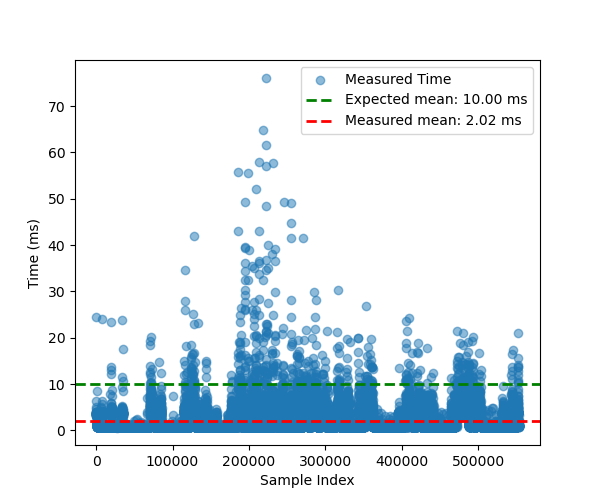
\includegraphics[width=1\linewidth]{figures/scatter_1000ssd_10ms.png}
    \caption{10ms event plot with 1ms SSD.} 
    \label{fig:1000ssd_10ms}
  \end{minipage}
  \hfill
  \begin{minipage}{0.5\textwidth}
    \centering
    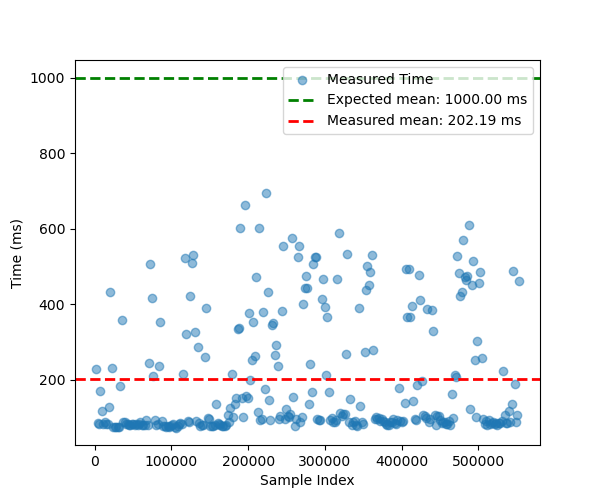
\includegraphics[width=1\linewidth]{figures/scatter_1000ssd_1s.png}
    \caption{1s event plot with 1ms SSD.} 
    \label{fig:1000ssd_1s}
  \end{minipage}
\end{figure}
From these plots, it became evident that there was a consistent deviation from real-time behavior. Specifically, the average time taken for each event was shorter than expected, suggesting an undesirable acceleration within the virtual environment. This deviation underscores the need for tighter synchronization between virtual and real-time execution to ensure accurate simulation results.

Interestingly, the timing deviation was consistent across different events, such as the 10ms and 100ms intervals. Upon further inspection of the SUTRunner's simulation code, we found that the system is driven by a timer interrupt managed by the "\textbf{ISR(Os\_TimerPfrtIsr)}" function, which is configured to trigger every 50 microseconds. Since all timing events are derived from this interrupt. This is why it`s expected that if one of the events goes slower the other events also go slower. When the SUTRunner was run with a simulation step duration of 1000 microseconds, the interrupt function was being called 20 times per simulation step, without any regard for real-time synchronization. This caused unadjusted virtual timing, making the simulation run faster than real time and preventing compensation for timing differences.


To address this, the initial solution involved reducing the simulation step duration to 50 microseconds, matching the interval of the interrupt function. This adjustment ensured that each simulation step directly aligned with the interrupt's timing. To account for the difference between virtual time and real time, we enabled a clock coupling thread on the SIL Kit. This thread checks after each simulation step if the virtual time is faster than the real time and waits until they equalize before proceeding to the next simulation step.

 \autoref{fig:50ssd_10ms} and \autoref{fig:50ssd_1s} show the results after implementing these modifications. Unfortunately, this approach did not yield the desired outcome. The events were slower than expected, likely due to the overhead associated with repeatedly calling the simulation function in very small time slices, as well as the additional tasks handled by the event loop. As a result, using 50-microsecond time slices proved ineffective for this architecture, leading to unsatisfactory performance.

\begin{figure}[h]
  \centering
  \begin{minipage}{0.49\textwidth}
    \centering
    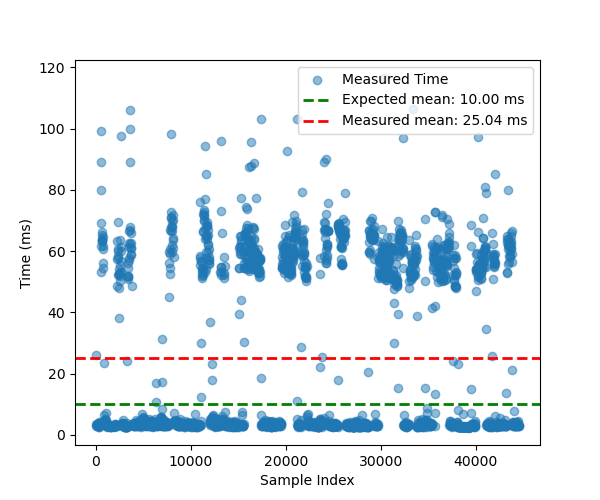
\includegraphics[width=1\linewidth]{figures/scatter_50ssd_10ms.png}
    \caption{10ms event Plot with 50$\mu$s SSD.} 
    \label{fig:50ssd_10ms}
  \end{minipage}
  \hfill
  \begin{minipage}{0.5\textwidth}
    \centering
    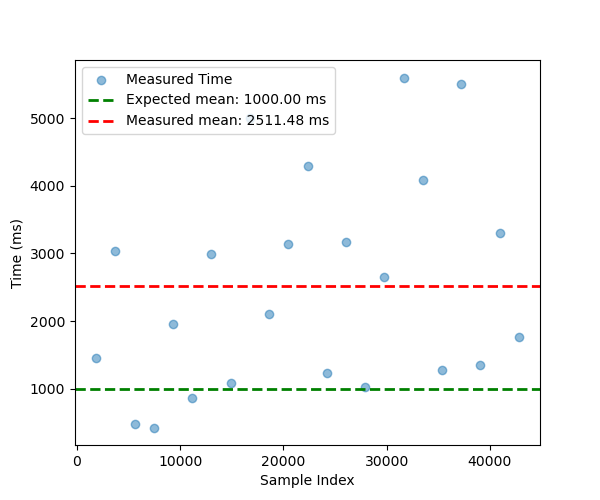
\includegraphics[width=1\linewidth]{figures/scatter_50ssd_1s.png}
    \caption{1s event Plot with 50$\mu$s SSD.} 
    \label{fig:50ssd_1s}
  \end{minipage}
\end{figure}

Considering that the smallest timing event in our simulation is 1ms, another strategy was to reconfigure the system by the timing of the interrupt function to be called every 1ms instead of 50 microseconds. This change would reduce the frequency of function calls and allow the simulation function to be called every 1000 microseconds, which is more aligned with the system's architecture. A clock coupling thread would still be necessary to maintain the balance between virtual and real time.

\autoref{fig:10ms_after}  and \autoref{fig:1s_after} show the results of this new approach for the 10ms and 1s events, respectively. The plots demonstrate that, after these adjustments, the virtual timing events now closely match real-time behavior. 

\begin{figure}[h]
  \centering
  \begin{minipage}{0.49\textwidth}
    \centering
    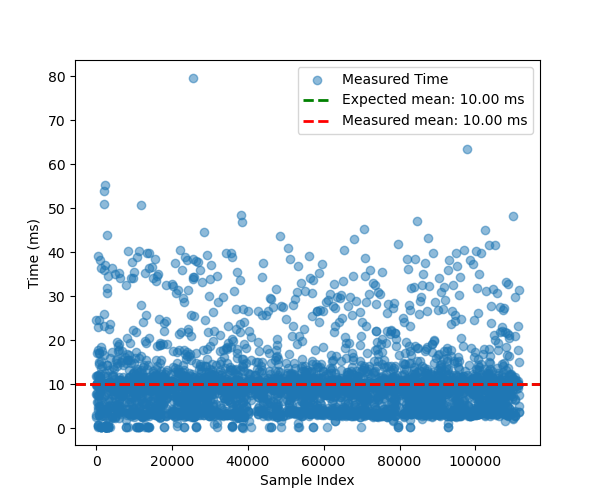
\includegraphics[width=1\linewidth]{figures/scatter_1000ssd_10ms_new.png}
    \caption{10ms event plot with 1ms SSD and 1ms timing interrupt.} 
    \label{fig:10ms_after}
  \end{minipage}
  \hfill
  \begin{minipage}{0.5\textwidth}
    \centering
    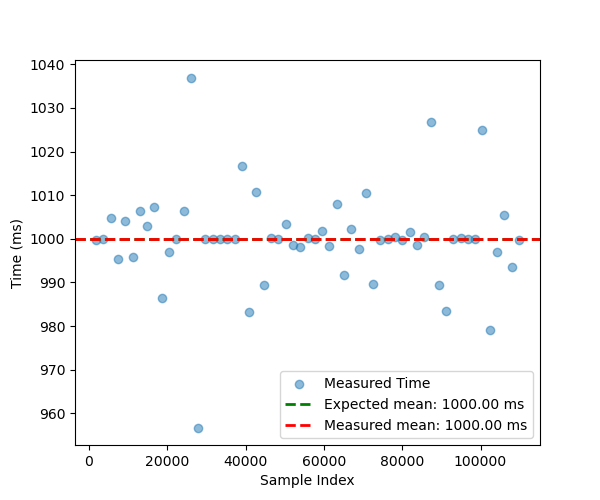
\includegraphics[width=1\linewidth]{figures/scatter_1000ssd_1s_new.png}
    \caption{1s event plot with 1ms SSD and 1ms timing interrupt.} 
    \label{fig:1s_after}
  \end{minipage}
\end{figure}


\begin{figure}[h]
  \centering
  \begin{minipage}{0.49\textwidth}
    \centering
    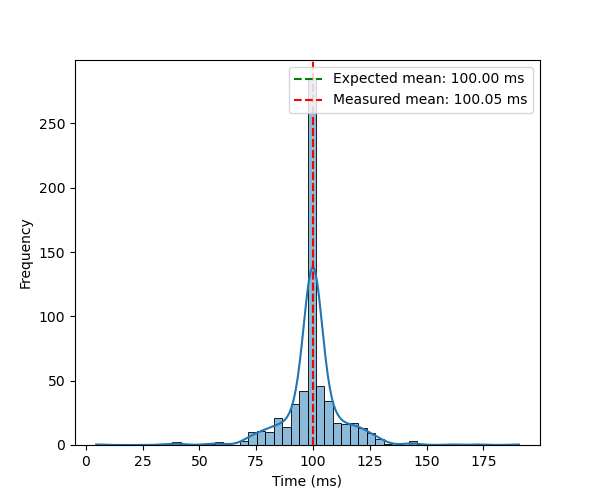
\includegraphics[width=1\linewidth]{figures/100ms_histogram_plot_new.png}
    \caption{100ms event histogram plot with 1ms SSD and 1ms timing interrupt.} 
    \label{fig:histogram_after}
  \end{minipage}
\end{figure}

\autoref{fig:histogram_after}  shows that the distribution of the 100ms timing event follows a normal distribution, with a mean of almost exactly 100ms, which is the expected and correct behavior.  These results confirm that, after implementing these modifications, the virtualized timing events now precisely align with the actual timing events on physical hardware, allowing for accurate and reliable simulation in the virtual environment.

\section{Correctness of the vECU}
To ensure the correctness of the virtual ECU (vECU), a series of real-world tests were conducted. These tests replicate the same procedures typically performed on a physical ECU, focusing on interactions between external components and the ECU, such as verifying the ability to install updates during the manufacturing process. The tests centered on sending Unified Diagnostic Services (UDS) requests from a testing tool to the vECU. 

To validate the vECU's response, a digital certificate was installed inside the vECU, and a series of UDS requests were sent to verify whether the system behaved as it would in a real ECU. A Python script was used to automate the process, sending the UDS requests and reading the certificate data from the vECU through UDS responses transmitted over the virtual CAN (vCAN) bus. The script was executed a hundred times to assess the robustness and consistency of the simulation. In each test iteration, the UDS requests were successfully delivered, and the vECU generated responses that matched the expected results, demonstrating the vECU’s correctness in handling diagnostic communication, just like a physical ECU would.

To demonstrate the virtual test environment's capability to execute a full set of tests for the BAC modules, four test suites, comprising 244 security-related tests, were run on both the virtual and hardware setups. The test suite contains robustness tests, this tests contain iterations of a feature, e.g. installing/deleting certificates 20 times. The tests executed in the virtual setup completed in 3 hours and 6 minutes, yielding identical results to those obtained on the hardware platform.

\section{Debugging}

A key objective of this project is not only to simulate the behavior of the ECU but also to enable a seamless debugging experience. Debugging in the virtual environment created for the vECU offers significant advantages over traditional real-time debugging on hardware.

In real-world testing with hardware, debugging usually involves connecting a hardware debugger to the ECU. This process is not only cumbersome but also limited by the hardware constraints. For example, real ECUs often have a finite number of hardware breakpoints—typically around eight. This limitation means that when debugging complex systems, the developer is restricted to setting a small number of breakpoints. Once the limit is reached, the debugger will refuse to set additional breakpoints, which can hinder the debugging process, especially when tracking down complex bugs that require observing multiple points in the code.

The virtualized environment for the vECU, however, overcomes these hardware constraints entirely. Using tools like GDB or the integrated debuggers in development environments, we can set an unlimited number of breakpoints in the virtual ECU without being restricted by hardware limitations. By being able to halt and inspect the execution at an infinite number of points, the virtual approach greatly enhances the debugging process, allowing more thorough and efficient issue resolution.
% !TeX root = ../main.tex

\chapter{Discussion}\label{chapter:discussion}


% Complete test coverage statistics
% Integerate to the CI
% CAN FD
% make Ecu-test use vertual time
% Level 4 vECU

This chapter reflects on the key findings presented in the evaluation and explores potential improvements, future implementations, and broader directions for enhancing the virtualized testing environment.

The results show that virtual timing events are now aligned with real-world timing, enabling accurate simulation of ECU behavior. The UDS requests from the test tool successfully retrieved certificates from the vECU, validating the accuracy of communication between the virtual and real components. Furthermore, the debugging process has become significantly more flexible, with the ability to set unlimited breakpoints—a substantial improvement over the hardware constraints of traditional ECU testing setups. This demonstrates that the virtualized test environment can effectively replicate the real test setup, providing an early and efficient way to test software modules before interacting with the physical ECU.

A crucial next step involves integrating the virtual ECU (vECU) into the Continuous Integration/Continuous Testing (CI/CT) pipeline. Currently, the system involves manually bundling various components, which can be cumbersome for developers who need to make changes to the software. Developers should be able to work directly with their source code in their repositories without having to switch between different environments. Integrating the virtualized test environment into the CI pipeline would streamline this process, allowing developers to automatically trigger tests, make adjustments, and continuously monitor results.

Looking ahead, one of the potential advancements in this area would be for testing tools, like ECU-Test, to enable time synchronization through a SIL Kit connector. This would allow all components of the virtual environment—such as the SutRunner and adapter—to be synchronized with the testing tool's virtual time. Although this feature is not yet available, if future versions of ECU-Test supported time synchronization, it could allow tests to be conducted in virtual time, significantly reducing testing duration. Currently, real-time testing can take days to complete, but with synchronized virtual time, the same tests could be completed much faster, allowing for more efficient testing and quicker software releases. 
% !TeX root = ../main.tex

\chapter{Conclusion}\label{chapter:conclusion}

This thesis explored the current state of virtualization techniques and examined their applicability to embedded systems testing. After evaluating various methods, Level 3 virtualization was selected for the project, given its suitability for separating software from hardware dependencies. Insights from real-time operating systems (RTOS) were used to understand similar virtualization techniques applied to areas closely aligned with this project.

The objective of this work was to create a virtualized testing environment that enables early testing and debugging of BAC software modules without the need for physical hardware. This was achieved by replacing the actual ECU with a virtual ECU (vECU), using the vVirtualtarget tool to virtualize different software components of the ECU. Three separate shared objects—representing the application, boot manager, and bootloader—were generated, each having its own simulation environment.

An adapter, vCan\_to\_silkit, was developed to facilitate communication between the vECU and the virtual CAN (vCAN) bus, allowing CAN messages to be exchanged with various test tools. The Silkit software was then used to integrate the vECU into a simulation environment, with the adapter acting as a participant.

A unified simulation was created, enabling the software components to share data and replicate the actual behavior of the ECU more accurately. The timing interrupt function was reconfigured to synchronize the virtual system with real-time behavior by calling it every millisecond.

With these adaptations, a virtualized testing environment was successfully developed, closely mirroring the behavior of a physical ECU. This environment not only provides early testing capabilities but also enhances debugging possibilities beyond the limitations of hardware-based testing.

% TODO: add more chapters here

\appendix{}

% TODO: appendix chapter
%\chapter{General Addenda}

If there are several additions you want to add, but they do not fit into the thesis itself, they belong here.

\section{Detailed Addition}

Even sections are possible, but usually only used for several elements in, e.g.\ tables, images, etc.

\chapter{Figures}
\section{Example 1}
\cmark
\section{Example 2}
\xmark

\microtypesetup{protrusion=false}
\listoffigures{}
% !TeX root = ../main.tex

\chapter*{List of Abbreviations}
\addcontentsline{toc}{chapter}{List of Abbreviations}

\begin{acronym}[BL]  % The longest acronym should go in the square brackets
  \acro{AmTS}{Automotive Test Suite}
  \acro{ASW}{Application Software}
  \acro{AUTOSAR}{Automotive Open System Architecture}
  \acro{BAC}{BMW AUTOSAR Core}
  \acro{BL}{Boot loader}
  \acro{BM}{Boot Manager}
  \acro{BSW}{Basic Software}
  \acro{CAN}{Controller Area Network}
  \acro{ECU}{Electronic Control Unit}
  \acro{MCAL}{Microcontroller Abstraction Layer}
  \acro{RTE}{Runtime Environment}
  \acro{RTOS}{Real-Time Operating Systems}
  \acro{SIL Kit}{Software-in-the-Loop Kit}
  \acro{SO}{Shared Object}
  \acro{SSD}{Simulation step duration}
  \acro{SUT}{System Under Test}
  \acro{UDS}{Unified Diagnostic Services}
  \acro{vCAN}{Virtual Controller Area Network}
  \acro{vECU}{Virtual Electronic Control Unit}
  \acro{VDK}{Virtualizer Development Kit}
\end{acronym}


%\listoftables{}
\microtypesetup{protrusion=true}
%\printglossaries
\printbibliography{}

\end{document}
